\subsection{Operator Learning}
\label{subsec:oplearning}
Here we describe how to learn operators $\operators$, assuming that the full set of predicates $\Psi$ is already learned~\cite{chitnis2021learning}.
This method makes two restrictions on the representation that together lead to very efficient operator learning (linear time in the number of transitions in $\D$).
First, for each $\controllerspec$ and each possible effect set pair $(\addeffects, \deleteeffects)$, there is at most one operator with that $(\controllerspec, \addeffects, \deleteeffects)$.
This restriction makes it impossible to learn multiple operators with different preconditions for the same controller and effect sets.
Second, each parameter in $\params$ must appear in $\params_{\controllerspec}, \addeffects$, or $\deleteeffects$.
This restriction prevents modeling ``indirect effects,'' where some object impacts the execution of a controller without its own state being changed.
Though these two restrictions are limiting, we are willing to accept them because predicate invention can compensate.
For example, an invented predicate can quantify out an object that does not appear in the controller or the effects, to capture indirect effects.
%\footnote{We see an example of this phenomenon in our experiments, where  in the Painting environment, a quantified predicate is learned to capture whether a box lid is open or closed, as a precondition of placing something into that box.}

With these restrictions established, we learn operators from our demonstrations $\D$ and predicates $\Psi$ in three steps. Note that each demonstration can be expressed as a sequence of transitions $\{(x, a, x')\}$, with $x, x' \in \X$ and $a \in \A$.
First, we use $\Psi$ to \textsc{Abstract} all states $x, x'$ in the demonstrations $\D$, creating a dataset of transitions $\{(s, a, s')\}$ with $s, s' \in \S_\Psi$.
Next, we partition these transitions using the following equivalence relation: $(s_1, a_1, s_1') \equiv (s_2, a_2, s_2')$ if the effects and partially specified controllers \emph{unify}, that is, if there exists a mapping between the objects such that $a_1$, $(s_1 - s_1')$, and $(s_1' - s_1)$ are equivalent to $a_2$, $(s_2 - s_2')$, and $(s_2' - s_2)$ respectively.
This partitioning step automatically determines the number of operators that will ultimately be learned: each equivalence class will induce one operator.
Furthermore, the parameters $\params$, controller tuple $\controllerspec$, and effects $(\addeffects, \deleteeffects)$ of the operators can now be established as follows.
For each equivalence class, we create $\params$ by selecting an arbitrary transition $(s, a, s')$ and replacing each object that appears in the controller or effects with a variable of the same type. This further induces a substitution $\delta: \params \to \O$ for the objects $\O$ in this transition; the $\controllerspec$, $\addeffects$, and $\deleteeffects$ are then created by applying $\delta$ to $a, (s' - s)$, and $(s - s')$ respectively.
By construction, for all other transitions $\tau$ in the same equivalence class, there exists an injective substitution $\delta_\tau$ under which the controller arguments and effects are equivalent to the newly created $\controllerspec, \addeffects$, and $\deleteeffects$.
We use these substitutions for the third and final step of operator learning: precondition learning.
For this, we perform an intersection over all abstract states in each equivalence class~\cite{bonet2019learning,chitnis2021learning,curtis2021discovering}: $\preconditions \gets \bigcap_{\tau=(s, \cdot, \cdot)} \delta^{-1}_\tau(s),$
where $\delta^{-1}_\tau(s)$  substitutes all occurrences of the objects in $s$ with the parameters in $\params$ following an inversion of $\delta_\tau$, and discards any atoms involving objects that are not in the image of $\delta_\tau$.
By this construction, only the parameters in $\params$ will be involved in $\preconditions$, as desired.
With $\params, \preconditions, \addeffects, \deleteeffects$, and $\controllerspec$ now established for each equivalence class, we have completed the operators $\operators$.

\textbf{Soundness.} We note that for any predicates $\Psi$, the operator learning procedure is \emph{sound}~\cite{konidaris2018skills} over the data, in the following sense: for each transition $\tau = (x, a, x')$, there exists some $\ground{\operator}$, a learned operator ground with objects in $x$, such that $F(\textsc{Abstract}(x, \Psi), \ground{\operator})$ is defined and equals $\textsc{Abstract}(x', \Psi)$. To see this, recall that $\tau$ belongs to an equivalence class, and that this equivalence class was used to learn an operator $\operator$.
Now, we show that the desired $\ground{\operator}$ is $\langle \operator, \delta_\tau \rangle$, where $\delta_\tau$ is the injective parameter-to-object substitution defined above. The $\ground{\controllerspec}$, $\ground{\addeffects}$, and $\ground{\deleteeffects}$ of $\ground{\operator}$ exactly equal those in $\tau$, by construction of the substitution $\delta_\tau$.
Additionally, because $\ground{\preconditions}$ was formed by taking an intersection of abstract states that included $\textsc{Abstract}(x, \Psi)$, it must be the case that $\ground{\preconditions} \subseteq \textsc{Abstract}(x, \Psi)$, since an intersection must be a subset of every constituent set.
By \defref{def:absmodel}, then, the statement is satisfied.
A corollary of this soundness property is that our learned abstractions are guaranteed to obey the semantics we defined in \secref{sec:representation} with respect to the training data.

As a byproduct of operator learning, we have also determined ``local'' datasets for each operator, with each transition in the respective equivalence class defining an example of the operator's preconditions, controller, and effects.
We will use these local datasets and the corresponding substitutions $\delta_\tau$ during sampler learning~\secref{subsec:samplerlearning}.

\subsection{Operator Learning Extended Example}

We conclude our discussion of operator learning with an extended example.
We start with a small toy dataset and use it to walk through each of the three steps in the procedure.

\textbf{Step 1: Generate Dataset.} In this example, our demonstrations contain four transitions, which are tuples $(x, a, x')$. For clarity, we will not write out the task-level states $x$ and $x'$. Additionally, for the sake of the example, we will assume that in this environment there is only one controller \texttt{C}, with no discrete arguments. We abstract these states with the predicate set $\Psi$ includes \texttt{Held}, \texttt{On}, \texttt{IsPurple}, \texttt{IsRed}, \texttt{IsGreen}, \texttt{IsStowable}, and \texttt{IsStowed}, which leads to four $(s, a, s')$ tuples:
\begin{enumerate}
    \item (\{\texttt{On}$(o_1, o_2)$, \texttt{On}$(o_2, o_3)$, \texttt{IsPurple}$(o_{1})$\}, \texttt{C}$(\theta_1)$,\{\texttt{Held}$(o_1)$, \texttt{On}$(o_2, o_3)$,
    \texttt{IsPurple}$(o_{1})$\})
    \item (\{\texttt{On}$(o_4, o_5)$, \texttt{On}$(o_{5}, o_{6})$, \texttt{IsRed}$(o_{4})$\}, \texttt{C}$(\theta_2)$,\{\texttt{Held}$(o_4)$, \texttt{On}$(o_{5}, o_{6})$, \texttt{IsRed}$(o_4)$\})
    \item (\{\texttt{Held}$(o_1)$, \texttt{IsStowable}$(o_1)$,
    \texttt{IsGreen}$(o_2)$\}, \texttt{C}$(\theta_3)$,\{\texttt{IsStowed}$(o_1)$, \texttt{IsStowable}$(o_1)$, \texttt{IsGreen}$(o_2)$\})
    \item (\{\texttt{Held}$(o_8)$, \texttt{IsStowable}$(o_8)$, \texttt{IsGreen}$(o_9)$\}, \texttt{C}$(\theta_4)$,\{\texttt{IsStowed}$(o_8)$, \texttt{IsStowable}$(o_8)$, \texttt{IsGreen}$(o_9)$\})
\end{enumerate}

Intuitively, the first and second transitions might occur when picking up an object ($o_1$ or $o_4$ respectively), while the third and fourth might occur when stowing an object ($o_1$ or $o_8$ respectively). We begin by noting that we can ignore the continuous parameters $\theta_i$ of \texttt{C}, since they do not matter for operator learning (they would be used in sampler learning).

\textbf{Step 2: Produce Equivalence Classes.} Recall that two transitions are in the same equivalence class if there exists a mapping between objects such that the controller, controller discrete arguments, and effects are equivalent. Since we only have one controller \texttt{C} with no discrete arguments in this example, we must only check for effect equivalence. The first transition has effects $(\addeffects, \deleteeffects) = (\{\texttt{Held}(o_1)\}, \{\texttt{On}(o_1,o_2)\})$, while the second has effects $(\addeffects, \deleteeffects) = (\{\texttt{Held}(o_4)\}, \{\texttt{On}(o_4,o_5)\})$. These can be unified with the mapping $\{o_1 \leftrightarrow o_4, o_2 \leftrightarrow o_5\}$. Similarly, the third transition has effects $(\addeffects, \deleteeffects) = (\{\texttt{IsStowed}(o_1)\}, \{\texttt{Held}(o_1)\})$, while the fourth has effects $(\addeffects, \deleteeffects) = (\{\texttt{IsStowed}(o_8)\}, \{\texttt{Held}(o_1)\})$. These can be unified with the mapping $\{o_1 \leftrightarrow o_8\}$.

Note that in this unification procedure, the atoms which were unchanged, such as \texttt{IsPurple}$(o_1)$, do not play a role. Furthermore, the fact that the objects are the same between transitions 1 and 3 is unimportant, because these transitions belong to different equivalence classes.

Selecting an arbitrary transition from each equivalence class and substituting objects with variables, we get the following:
\begin{itemize}
    \item Equivalence class 1:
    \begin{itemize}
    \item $\params$: [\texttt{?x}, \texttt{?y}] \item $\addeffects$: \{\texttt{Held(?x)}\} \item $\deleteeffects$: \{\texttt{On(?x, ?y)}\} \item $\controllerspec$: $\langle$ \texttt{C}, [] $\rangle$
    \item Transitions contained: 1 and 2
    \item $\delta_1$ (substitution for transition 1): \{\texttt{?x} $\to o_1$, \texttt{?y} $\to o_2$\}
    \item $\delta_2$ (substitution for transition 2): \{\texttt{?x} $\to o_4$, \texttt{?y} $\to o_5$\}
    \end{itemize}
    \item Equivalence class 2:
    \begin{itemize}
    \item $\params$: [\texttt{?z}] \item $\addeffects$: \{\texttt{IsStowed(?z)}\} \item $\deleteeffects$: \{\texttt{Held(?z)}\} \item $\controllerspec$: $\langle$ \texttt{C}, [] $\rangle$
    \item Transitions contained: 3 and 4
    \item $\delta_3$ (substitution for transition 3): \{\texttt{?z} $\to o_1$\}
    \item $\delta_4$ (substitution for transition 4): \{\texttt{?z} $\to o_8$\}
    \end{itemize}
\end{itemize}

Note that the parameter list $\params$ for each equivalence class contains all parameters that appear in $\params_{\controllerspec}, \addeffects$, or $\deleteeffects$.

\textbf{Step 3: Learn Operator Preconditions.} We now have all the ingredients of the operators except for their preconditions. For each transition in each equivalence class, we first discard any atom from the abstract state $s$ which involves objects \emph{not} in the image of that transition's substitution $\delta$. For instance, the first transition has $\delta_1 =$ \{\texttt{?x} $\to o_1$, \texttt{?y} $\to o_2$\}. The image is $\{o_1, o_2\}$, which excludes $o_3$. This means that the atom \texttt{On}$(o_2, o_3)$ is discarded from $s$.

After discarding atoms appropriately, we end up with these abstract states for each transition:
\begin{enumerate}
    \item \{\texttt{On}$(o_1, o_2)$, \texttt{IsPurple}$(o_{1})$\}
    \item \{\texttt{On}$(o_4, o_5)$, \texttt{IsRed}$(o_{4})$\}
    \item \{\texttt{Held}$(o_1)$, \texttt{IsStowable}$(o_1)$\}
    \item \{\texttt{Held}$(o_8)$, \texttt{IsStowable}$(o_8)$\}
\end{enumerate}

Now, the preconditions for each equivalence class are obtained by applying each $\delta_i^{-1}$ to these abstract states and taking intersections. This produces the final operator set $\operators$, which does not contain any extraneous atoms related to object color:

\begin{itemize}
    \item Operator 1 (from equivalence class 1):
    \begin{itemize}
    \item $\params$: [\texttt{?x}, \texttt{?y}]
    \item $\preconditions$: \{\texttt{On(?x, ?y)}\}
    \item $\addeffects$: \{\texttt{Held(?x)}\} \item $\deleteeffects$: \{\texttt{On(?x, ?y)}\} \item $\controllerspec$: $\langle$ \texttt{C}, [] $\rangle$
    \end{itemize}
    \item Operator 2 (from equivalence class 2):
    \begin{itemize}
    \item $\params$: [\texttt{?z}]
    \item $\preconditions$: \{\texttt{Held(?z)}, \texttt{IsStowable(?z)}\}
    \item $\addeffects$: \{\texttt{IsStowed(?z)}\} \item $\deleteeffects$: \{\texttt{Held(?z)}\} \item $\controllerspec$: $\langle$ \texttt{C}, [] $\rangle$
    \end{itemize}
\end{itemize}

\subsection{Learning Samplers}
\label{subsec:samplerlearning}

The role of a sampler $\sampler \in \samplers$ is to \emph{refine} its associated operator $\operator$, suggesting continuous parameters of actions that will transition the environment from a state where the preconditions hold to a state where the effects follow.
Recall that a sampler $\sampler : \X \times \O^{|\params|} \to \Delta(\Theta)$ defines a conditional distribution $P(\theta \mid x, o_1, \dots, o_k)$, where $\theta$ are continuous parameters for the controller $C$ in $\operator$, and $(o_1, \ldots, o_k)$ represent a set of objects that could be used to ground $\omega$, with $|\params| = k$.
Using the same demonstration dataset $\D$, we learn samplers of the following form, one per operator: $$\sampler(x, o_1, \dots, o_k) = r_\sampler(x[o_1] \oplus \cdots \oplus x[o_k]),$$
where $x[o]$ denotes the feature vector for $o$ in $x$, the $\oplus$ denotes concatenation, and $r_\sampler$ is the model to be learned.

To learn samplers, we use the local datasets created during operator learning (\secref{subsec:oplearning}), to create datasets for supervised sampler learning, with one dataset per sampler.
Consider any (non-abstract) transition $\tau = (x, a, \cdot)$ in the equivalence class associated with an operator $\omega$.
To create a datapoint for the associated sampler, we can reuse the substitution $\delta_\tau$ found during operator learning to create an input vector $x[\delta_\tau(v_1)] \oplus \cdots \oplus x[\delta_\tau(v_k)]$, where $(v_1, \dots, v_k) = \params$.
The corresponding output for supervised learning is the continuous parameter vector $\theta$ in the action $a$.

With these datasets created, one could use any method for multidimensional distributional regression to learn each $r_\sampler$.
In this work, we learn two neural networks to parameterize each sampler.
The first neural network takes in $x[o_1] \oplus \cdots \oplus x[o_k]$ and regresses to the mean and covariance matrix of a Gaussian distribution over $\theta$; here, we are assuming that the desired distribution has nonzero measure, but the covariances can be arbitrarily small in practice.
This neural network is a sampler in its own right, but its expressive power is limited, e.g., to unimodal distributions.
To improve representational capacity, we learn a second neural network that takes in $x[o_1] \oplus \cdots \oplus x[o_k]$ \emph{and} $\theta$, and returns true or false.
This classifier is then used to rejection sample from the first network.
To create negative examples, we use all transitions $\tau'$ such that the controller in $\tau'$ matches that in $\controllerspec$, but the effects in $\tau'$ are different from $(\addeffects, \deleteeffects)$.

\subsection{Predicate Grammar Details}
\label{app:grammar}

Here we detail the grammar over predicate candidates used in our experiments.
Note that the grammar is the same for all environments (up to the object types and goal predicates).

\begin{tightlist}
\item The base grammar includes two kinds of predicates: all the goal predicates $\Psi_G$, and \emph{single-feature inequality classifiers}. These inequality classifiers are less-than-or-equal-to expressions that compare a constant against an individual feature dimension from $\{1, \ldots, d(\type)\}$, for some object type $\type \in \types$. For the constant, we consider an infinite stream of numbers in the pattern $0.5, 0.25, 0.75, 0.125, 0.375, 0.625, 0.875, \ldots$, which represent \emph{normalized} values of the feature, based on the range of values it takes on across all states in the dataset $\D$. We use this pattern because we want our grammar to describe an infinite stream of classifiers, starting from the median values in $\D$. As an example, a type \texttt{block} might have a feature dimension corresponding to its \texttt{size}, and a classifier could be \texttt{block.size $\leq$ 0.5}. All goal predicates have cost 0. All single-feature inequality classifiers have cost computed based on the normalized constant, with cost 0 for constant $0.5$, cost 1 for constants $0.25$ and $0.75$, cost 2 for constants $0.125$, $0.375$, $0.625$, $0.875$, etc.
\item We include all negations of predicates in the base grammar. Negating a predicate adds a cost of 1.
\item We include two types of universally quantified predicates over the predicates thus far: (1) quantifying over all variables, and (2) quantifying over all but one variable. An example of the first is \texttt{P()} = $\forall$ \texttt{?x}, \texttt{?y} . \texttt{On}(\texttt{?x}, \texttt{?y}), while an example of the second is \texttt{P(?y)} = $\forall$ \texttt{?x} . \texttt{On}(\texttt{?x}, \texttt{?y}). Universally quantifying adds a cost of 1.
\item We include all negations of universally quantified predicates. Negating a predicate adds a cost of 1.
\item Following prior work~\cite{curtis2021discovering}, we prune out candidate predicates if they are equivalent to any previously enumerated predicate, in terms of all groundings that hold in every state in the dataset $\D$. Finally, we discard the goal predicates $\Psi_G$ from the grammar, since they are included in every candidate predicate set  $\Psi$ of our search already.
\end{tightlist}


\subsection{Additional Environment Details}
\label{app:details}

\begin{tightlist}
    \item \textbf{PickPlace1D.} In this toy environment, a robot must pick blocks and place them onto target regions along a table surface. All pick and place poses are in a 1D line. The three object types are block, target, and robot. Blocks and targets have two features for their pose and width, and robots have one feature for the gripper joint state. The block widths are larger than the target widths, and the goal requires each block to be placed so that it completely covers the respective target region, so $\Psi_G = \{\texttt{Covers}\}$, where \texttt{Covers} is an arity-2 predicate. There is only one controller, \texttt{PickPlace}, with no discrete arguments; its $\Theta$ is a single real number denoting the location to perform either a pick or a place, depending on the current state of the robot's gripper. Each action updates the state of at most one block, based on whether any is in a small radius from the continuous parameter $\theta$. Both training tasks and evaluation tasks involve 2 blocks, 2 targets, and 1 robot. In each task, with 75\% probability the robot starts out holding a random block; otherwise, both blocks start out on the table. Evaluation tasks require 1-4 actions to solve. This environment was established by~\citet{silver2021learning}, but that work involved manually defined state abstractions, which we do not provide in this paper.
    \item \textbf{Blocks.} In this environment, a robot in 3D must interact with blocks on a table to assemble them into towers. This is a robotics adaptation of the blocks world domain in AI planning. The two object types are block and robot. Blocks have four features: an x/y/z pose and a bit for whether it is currently grasped. Robots have four features: x/y/z end effector pose and the (symmetric) value of the finger joints. The goals involve assembling towers, so $\Psi_G = \{\texttt{On}, \texttt{OnTable}\}$, where the former has arity 2 and describes one block being on top of another, while the latter has arity 1. There are three controllers: \texttt{Pick}, \texttt{Stack}, and \texttt{PutOnTable}. \texttt{Pick} is parameterized by a robot and a block to pick up. \texttt{Stack} is parameterized by a robot and a block to stack the currently held one onto. \texttt{PutOnTable} is parameterized by a robot and a 2D place pose representing normalized coordinates on the table surface at which to place the currently held block. Training tasks involve 3 or 4 blocks, while evaluation tasks involve 5 or 6 blocks; all tasks have 1 robot. In all tasks, all blocks start off in collision-free poses on the table. Evaluation tasks require 2-20 actions to solve. This environment was established by~\citet{silver2021learning}, but that work involved manually defined state abstractions, which we do not provide in this paper.
    \item \textbf{Painting.} In this challenging environment, a robot in 3D must pick, wash, dry, paint, and place widgets into either a box or a shelf, as specified by the goal. The five object types are widget, box, shelf, box lid, and robot. Widgets have eight features: an x/y/z pose, a dirtiness level (requiring washing), a wetness level (requiring drying), a color, a bit for whether it is currently grasped, and the 1D gripper rotation with which it is grasped if so. Boxes and shelves have one feature for their color. Box lids have one feature for whether or not they are open. Robots have one feature for the gripper joint state. The goals involve painting the widgets to be the same color as either a box or a shelf, and then placing each widget into the appropriate one, so $\Psi_G = \{\texttt{InBox}, \texttt{InShelf}, \texttt{IsBoxColor}, \texttt{IsShelfColor}\}$, all of which have arity 2 (a widget, and either a box or a shelf). There are two physical constraints in this environment: (1) placing into a box can only succeed if the robot is top-grasping a widget, while placing into a shelf can only succeed if the robot is side-grasping it; (2) a box can only be placed into if its respective lid is open. There are six controllers: \texttt{Pick}, \texttt{Wash}, \texttt{Dry}, \texttt{Paint}, \texttt{Place}, and \texttt{OpenLid}. All six are discretely parameterized by a robot argument; \texttt{Pick} is additionally parameterized by a widget to pick up, and \texttt{OpenLid} by a lid to open. \texttt{Pick} has 4 continuous parameters: a 3D grasp pose delta from that widget's center of mass, and a gripper rotation. \texttt{Wash}, \texttt{Dry}, and \texttt{Paint} have 1 continuous parameter each: the amount of washing, the amount of drying, and the desired new color, respectively. \texttt{Place} has 3 continuous parameters: a 3D place pose corresponding to where the currently held widget should be placed. Training tasks involve 2 or 3 widgets, while evaluation tasks involve 3 or 4 blocks; all tasks have 1 box, 1 shelf, and 1 robot. In each task, with 50\% probability the robot starts out holding a random widget; otherwise, all widgets start out on the table. Also, in each task, with 30\% probability the box lid starts out open. Evaluation tasks require 11-25 actions to solve. This environment was established by~\citet{silver2021learning}, but that work involved manually defined state abstractions, which we do not provide in this paper.
    \item \textbf{Tools.} In this challenging environment, a robot operating on a 2D table surface must assemble contraptions by fastening screws, nails, and bolts, using a provided set of screwdrivers, hammers, and wrenches respectively. This environment has physical constraints outside the scope of our predicate grammar, and therefore tests the learner's ability to be robust to an insurmountable lack of downward refinability. The eight object types are contraption, screw, nail, bolt, screwdriver, hammer, wrench, and robot. Contraptions have two features: an x/y pose. Screws, nails, bolts, and the three tools have five features: an x/y pose, a shape, a size, and a bit indicating whether it is held. Robots have one feature for the gripper joint state. The goals involve fastening the screws, nails, and bolts onto target contraptions, so $\Psi_G$ includes \texttt{ScrewPlaced}, \texttt{NailPlaced}, \texttt{BoltPlaced}, \texttt{ScrewFastened}, \texttt{NailFastened}, and \texttt{BoltFastened}. The first three have arity 2 (a screw/nail/bolt and which contraption it is placed on); the last three have arity 1. There are three physical constraints in this environment: (1) a screwdriver can only be used to fasten a screw if its shape is close enough to that of the screw; (2) some screws have a shape that does not match any screwdriver's, and so these screws must be fastened by hand; (3) the three tools cannot be picked up if their sizes are too large. There are eleven controllers: \texttt{Pick\{Screw, Nail, Bolt, Screwdriver, Hammer, Wrench\}}, \texttt{Place}, \texttt{FastenScrewWithScrewdriver}, \texttt{FastenScrewByHand}, \texttt{FastenNailWithHammer}, and \texttt{FastenBoltWithWrench}. All eleven are discretely parameterized by a robot argument; \texttt{Pick} controllers are additionally parameterized by an object to pick up, and \texttt{Fasten} controllers by a screw/nail/bolt and tool (except \texttt{FastenScrewByHand}, which does not have a tool argument). \texttt{Place} has 2 continuous parameters: a 2D place pose corresponding to where the currently held object should be placed, which can be either onto the table or onto a contraption (only if the currently held object is not a tool). Training tasks involve 2 screws/nails/bolts and 2 contraptions, while evaluation tasks involve 2 or 3 screws/nails/bolts and 3 contraptions; all tasks have 3 screwdrivers, 2 hammers, 1 wrench, and 1 robot. Evaluation tasks require 7-20 actions to solve.
\end{tightlist}


\subsection{Additional Experimental Details}
\label{app:additional-experimental-details}
All experiments were conducted on a quad-core Intel Xeon Platinum 8260 processor.
All sampler neural networks are fully connected, with two hidden layers of size 32 each, and trained with the Adam optimizer~\cite{kingma2014adam} for 1K epochs using learning rate 1e-3. The regressor networks are trained to predict a mean and covariance matrix of a multivariate Gaussian; this covariance matrix is restricted to be diagonal and PSD with an exponential linear unit~\cite{clevert2015fast}.
For training the classifier networks, we subsample data to ensure a 1:1 balance between positive and negative examples.
All AI planning heuristics are implemented using Pyperplan~\cite{pyperplan}; all experiments use the LMCut heuristic unless otherwise specified.
The planning parameters are $n_{\text{abstract}} = 1000$ for Tools and $8$ for the other environments, and $n_{\text{samples}} = 1$ for Tools and $10$ for the other environments.


\subsection{Additional Experimental Results}
\label{app:results}

\tabref{tab:learningtimeresults} provides learning times for all experiments.
Tables \ref{tab:allsuccresults}, \ref{tab:allnodesresults}, and \ref{tab:alltimeresults} report success rates, nodes created, and wall-clock time respectively for all evaluation tasks.

\figref{fig:decomposition} analyzes the two main features used by our surrogate objective function. See caption for further description.


\begin{figure*}[b]
  \centering
    \noindent
    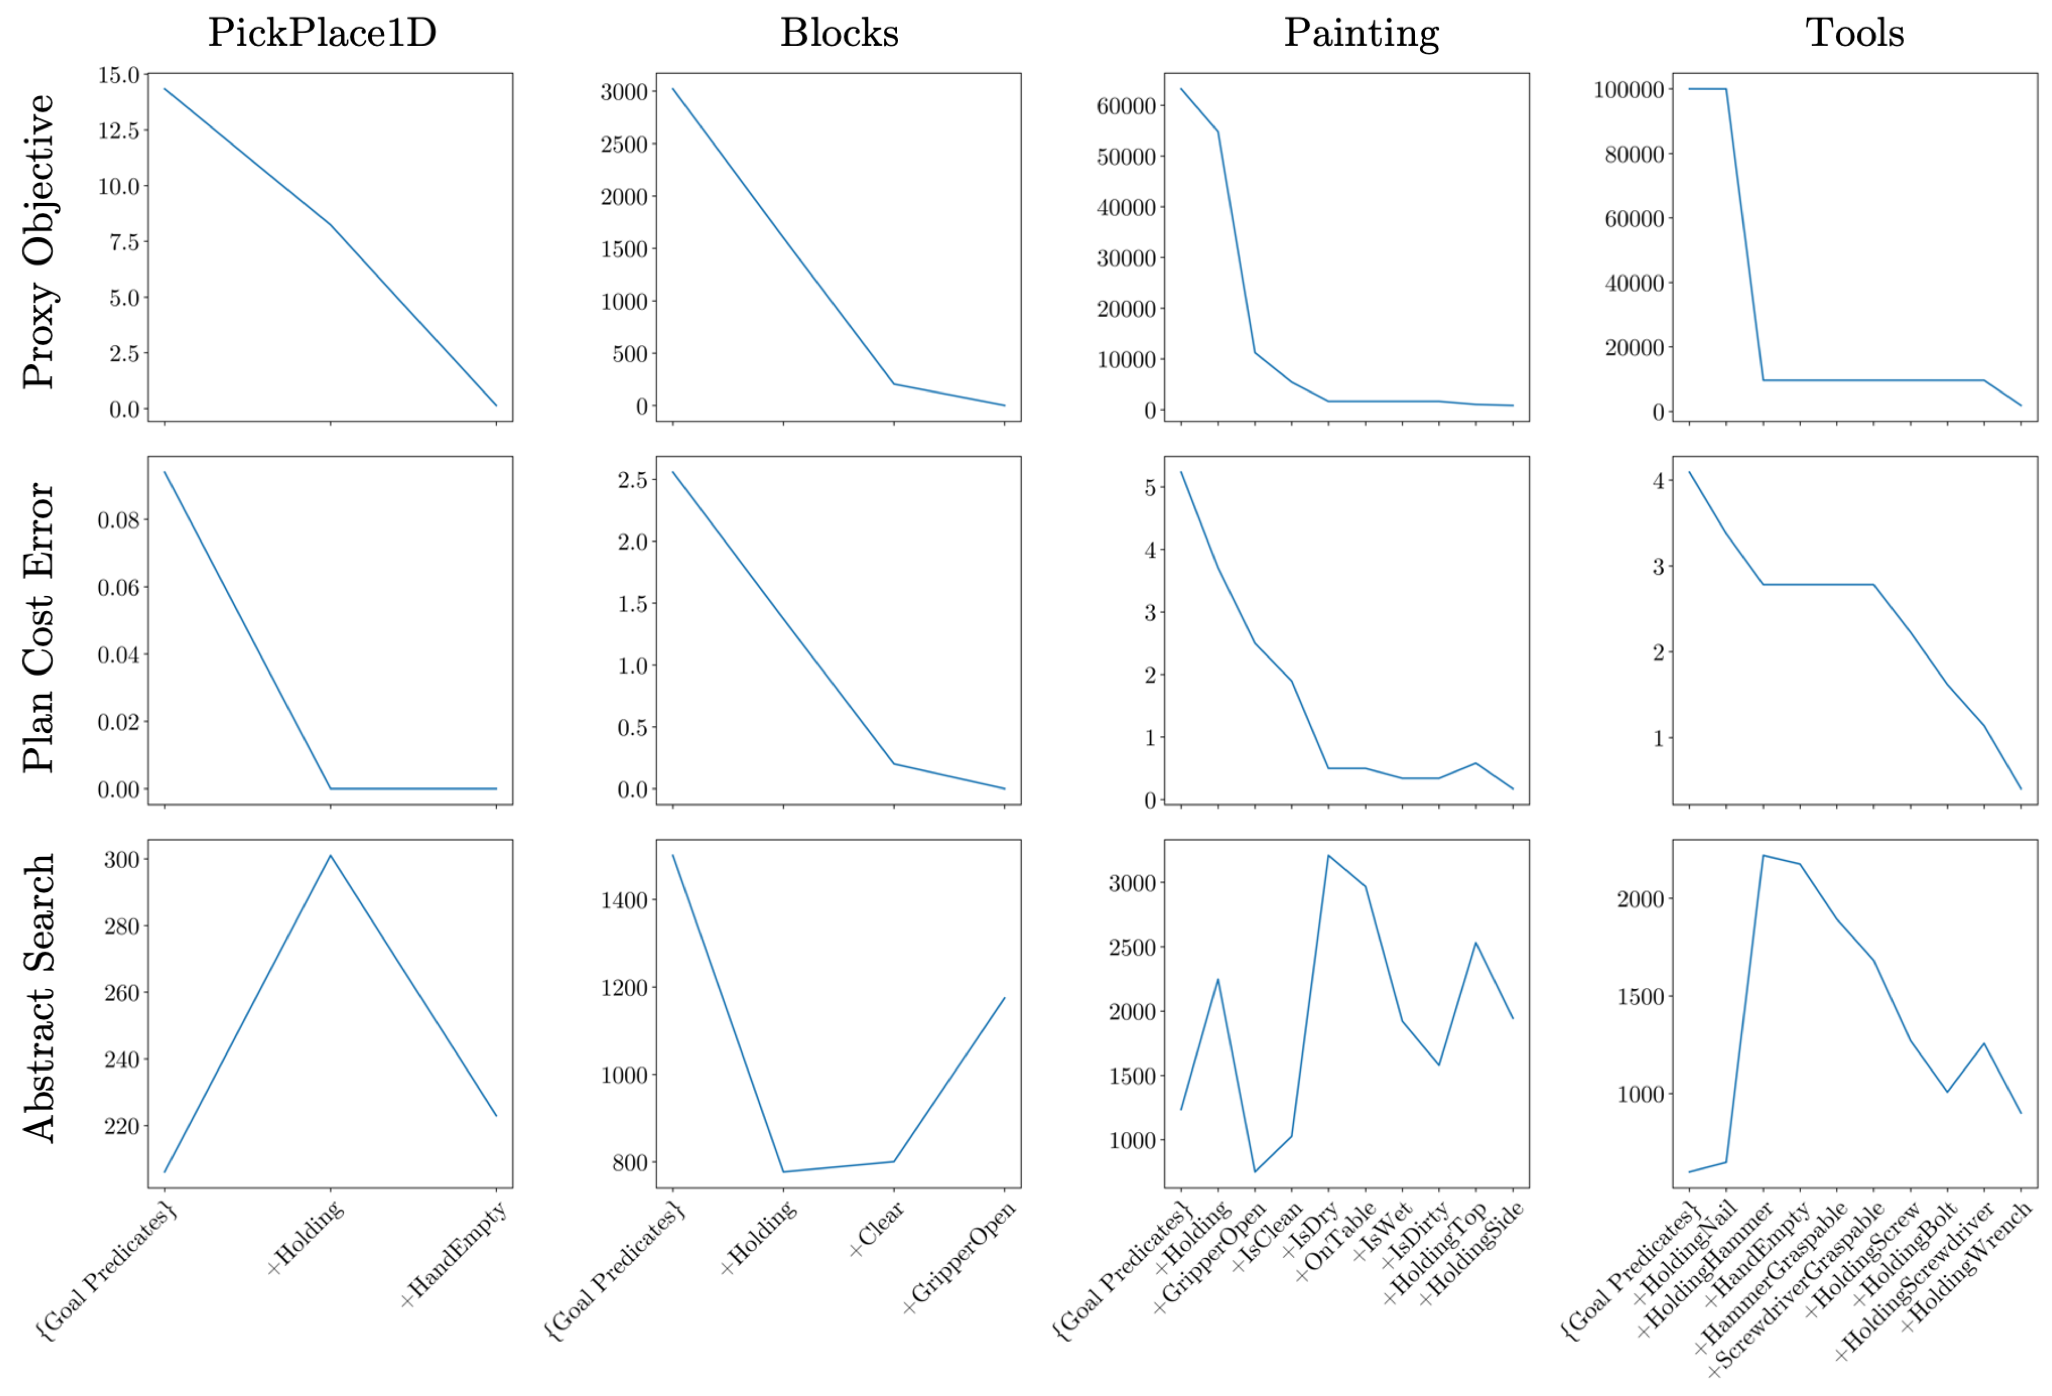
\includegraphics[width=\textwidth]{figures/decomposition_plots.png}
    \caption{\textbf{Decomposing the surrogate objective.} In these plots, each column corresponds to one environment. The x-axes correspond to sets of manually designed predicates. The predicate sets grow in size from left to right, starting with the goal predicates alone, adding one predicate at each tick mark, and concluding with the full set of manual predicates for the respective environment. The order that the predicates are added was determined by hill climbing with respect to the surrogate objective. The top row shows the surrogate objective itself; the middle row shows the plan cost error $|\textsc{Cost}(\hat{\pi}) - \textsc{Cost}(\pi^*)|$ minimized over the first 8 skeletons generated by abstract search; and the bottom row shows the total number of nodes created by the abstract search (our measure of abstract search time), cumulative over the 8 skeletons. \emph{There are two key takeaways from this plot.} (1) The surrogate objective (first row) monotonically decreases in all environments; this smoothness makes local search over candidate predicate sets an attractive option. (2) Neither of the two components that make up the surrogate objective --- plan cost error (second row) or abstract search time (third row) --- has the same monotonically decreasing property on its own, suggesting that both parts are necessary for making our predicate invention pipeline work. All results are means over 10 seeds.}
  \label{fig:decomposition}
\end{figure*}

We now go through each of our four environments, providing an example of learned predicates and operators from a single seed randomly chosen among successful ones.
We also provide additional statistics for our main method, to supplement the other results we have provided.
Note that the evaluation plan length statistics are averaged over both 10 seeds and 50 evaluation tasks per seed, \emph{with standard deviations over seed only}.

\subsubsection{PickPlace1D}

Statistics for our main method, averaged over 10 random seeds (standard deviations parenthesized):
\begin{tightlist}
\item Average number of predicates in $\Psi$ (both invented and goal predicates): 5.9 (0.54)
\item Average number of operators in $\operators$: 2.1 (0.3)
\item Average plan length during evaluation: 2.44 (0.09)
\end{tightlist}

See \figref{fig:pickplace1dlearned} for example learned predicates and operators for a randomly chosen successful seed.


\subsubsection{Blocks}
Statistics for our main method, averaged over 10 random seeds (standard deviations parenthesized):
\begin{tightlist}
\item Average number of predicates in $\Psi$ (both invented and goal predicates): 6.0 (0.0)
\item Average number of operators in $\operators$: 4.0 (0.0)
\item Average plan length during evaluation: 9.17 (0.69)
\end{tightlist}

See \figref{fig:blockslearned} for example learned predicates and operators for a randomly chosen successful seed.


\subsubsection{Painting}
Statistics for our main method, averaged over 10 random seeds (standard deviations parenthesized):
\begin{tightlist}
\item Average number of predicates in $\Psi$ (both invented and goal predicates): 22.1 (1.45)
\item Average number of operators in $\operators$: 11.2 (0.6)
\item Average plan length during evaluation: 14.76 (0.29)
\end{tightlist}

See Figures \ref{fig:paintinglearned1} and \ref{fig:paintinglearned2} for example learned predicates and operators for a randomly chosen successful seed.



\subsubsection{Tools}
Statistics for our main method, averaged over 10 random seeds (standard deviations parenthesized):
\begin{tightlist}
\item Average number of predicates in $\Psi$ (both invented and goal predicates): 27.4 (4.39)
\item Average number of operators in $\operators$: 17.8 (0.98)
\item Average plan length during evaluation: 10.1 (0.12)
\end{tightlist}

See Figures \ref{fig:toolslearned1} and \ref{fig:toolslearned2} for example learned predicates and operators for a randomly chosen successful seed.


\begin{table}
\begin{center}
\scriptsize
\begin{tabular}{| l | c | c | c | c | c | c | }
	\hline
	\multicolumn{1}{|c|}{} &\multicolumn{3}{c|}{\bf{Ours}} &
	\multicolumn{3}{c|}{\bf{Manual}} \\
	\hline
	\bf{Heuristic} &
	{Succ} & {Node} & {Time}&
	{Succ} & {Node} & {Time}\\
	\hline
	LMCut & 98.4 & 2949 & 0.296 & 98.6 & 2941 & 0.251 \\
	hAdd & 98.6 & 121.6 & 0.115 & 97.8 & 3883 & 0.235 \\\hline
	\end{tabular}
	\caption{\textbf{Varying planning heuristic}. See text for details.}
	\label{tab:varying-heuristic}
\end{center}
\end{table}

\begin{table*}[t]
	\centering
	\scriptsize
	
	\begin{tabular}{| l | c || c | c | c | c | c || c | c | }
	\hline
	{\bf{Environment}} &{\bf{Ours}} &
	{\bf{Bisimulation}} &
	{\bf{Branching}} &
	{\bf{Boltzmann}} &
	{\bf{GNN Sh}} &
	{\bf{GNN MF}} &
	{\bf{Manual}} &
	{\bf{No Invent}} \\
	\hline
	PickPlace1D & 625 (134) & 176 (3) & 219 (145) & 264 (17) & 1951 (85) & 1951 (85) & 177 (147) & 66 (0) \\
	Blocks & 10237 (853) & 800 (44) & 1561 (98) & 9798 (1688) & 4047 (209) &4047 (209) & 102 (5) & 84 (2) \\
	Painting & 18395 (28153) & 872 (380) & 2883 (144) & 9457 (3421) & 9185 (166) & 9185 (166) & 565 (457) & 260 (2) \\
	Tools & 18666 (2815) & 573 (20) & 5524 (747) & 9716 (1000) & 7362 (197) & 7362 (197) & 167 (3) & 141 (3) \\\hline
	\end{tabular}
	\caption{\textbf{Learning times in seconds for all experiments}. All numbers are means over 10 seeds, with standard deviations in parentheses. For the GNN-based methods, learning time encompasses training the neural networks. For the other methods, learning time encompasses learning predicates, operators, and samplers (i.e., all components of the abstraction). Even though our main method performs well (Ours), this does come at the cost of increased learning time (although the learning is purely offline). Note that the Manual approach only manually specifies a \emph{state} abstraction (predicates); operators and samplers must still be learned, contributing to the non-zero learning time. Thus, comparing Ours and Manual shows that the large majority of learning time in our system is spent on predicate invention.}
	\label{tab:learningtimeresults}
\end{table*}
\begin{table*}[t]
	\centering
	\scriptsize
	
	\begin{tabular}{| l | c || c | c | c | c | c | c || c | c | c | }
	\hline
	{\bf{Environment}} &{\bf{Ours}} &
	{\bf{Bisimulation}} &
	{\bf{Branching}} &
	{\bf{Boltzmann}} &
	{\bf{GNN Sh}} &
	{\bf{GNN MF}} &
	{\bf{Random}} &
	{\bf{Manual}} &
	{\bf{Down Eval}} &
	{\bf{No Invent}} \\
	\hline
	PickPlace1D & 98.6 (1.6) & 98.4 (1.5) & 98.4 (1.5) & 98.4 (1.5) & 100.0 (0.0) & 15.2 (8.7) & 19.2 (5.4) & 98.4 (1.5) & 98.6 (1.6) & 39.6 (4.8) \\
	Blocks & 98.4 (1.5) & 19.0 (4.9) & 98.4 (1.5) & 64.8 (23.5) & 27.8 (4.0) & 35.4 (6.8) & 0.6 (0.9) & 98.6 (1.6) & 98.2 (1.4) & 3.2 (2.0) \\
	Painting & 100.0 (0.0) & 0.0 (0.0) & 20.2 (7.1) & 88.6 (29.7) & 59.2 (17.3) & 0.6 (0.9) & 0.0 (0.0) & 99.6 (0.8) & 98.8 (1.8) & 0.0 (0.0) \\
	Tools & 96.8 (4.7) & 26.2 (5.6) & 75.8 (8.4) & 64.2 (3.7) & 25.6 (9.0) & 22.0 (8.9) & 0.0 (0.0) & 100.0 (0.0) & 42.8 (10.4) & 0.0 (0.0) \\\hline

	\end{tabular}
	\caption{\textbf{Percentage of evaluation tasks solved for all experiments}. All numbers are means over 10 seeds, with 50 evaluation tasks per seed, and with standard deviations in parentheses.}
	\label{tab:allsuccresults}
\end{table*}
\begin{table*}[t]
	\centering
	\scriptsize
	
	\begin{tabular}{| l | c || c | c | c || c | c | c | }
	\hline
	{\bf{Environment}} &{\bf{Ours}} &
	{\bf{Bisimulation}} &
	{\bf{Branching}} &
	{\bf{Boltzmann}} &
	{\bf{Manual}} &
	{\bf{Down Eval}} &
	{\bf{No Invent}} \\
	\hline
	PickPlace1D & 4.8 (0.2) & 4.7 (0.2) & 4.7 (0.2) & 5.3 (0.2) &    6.5 (0.3) & 4.8 (0.2) & 14.1 (4.0) \\
	Blocks & 2948.5 (1293.2) & 46.9 (18.0) & 2948.5 (1293.2) & 7844.0 (6655.4) &    2940.5 (1299.1) & 2948.5 (1293.2) & 427.7 (83.7) \\
	Painting & 501.8 (180.0) & \;\;\;-- & 876.6 (509.7) & 4008.8 (3851.3) &    2607.5 (1117.2) & 489.0 (190.2) & \;\;\;-- \\
	Tools & 1897.2 (1404.0) & 5247.7 (2560.6) & 167.8 (78.4) & 909.9 (174.1) &    4770.9 (886.8) & 152.5 (27.6) & \;\;\;-- \\\hline
	\end{tabular}
	\caption{\textbf{Number of nodes created by abstract search during planning in evaluation tasks}. All numbers are means over \emph{solved tasks only} across 10 seeds, with 50 evaluation tasks per seed, and with standard deviations in parentheses.}
	\label{tab:allnodesresults}
\end{table*}
\begin{table*}[t]
	\centering
	\scriptsize
	
	\begin{tabular}{| l | c || c | c | c | c | c | c || c | c | c | }
	\hline
	{\bf{Environment}} &{\bf{Ours}} &
	{\bf{Bisimulation}} &
	{\bf{Branching}} &
	{\bf{Boltzmann}} &
	{\bf{GNN Sh}} &
	{\bf{GNN MF}} &
	{\bf{Random}} &
	{\bf{Manual}} &
	{\bf{Down Eval}} &
	{\bf{No Invent}} \\
	\hline
	PickPlace1D & 0.006 (0.0) & 0.006 (0.0) & 0.006 (0.0) & 0.005 (0.0) & 0.436 (0.1) & 0.014 (0.0) & 0.004 (0.0) & 0.045 (0.0) & 0.008 (0.0) & 1.369 (0.6) \\
	Blocks & 0.296 (0.1) & 0.158 (0.1) & 0.284 (0.1) & 0.954 (0.3) & 0.138 (0.1) & 0.249 (0.1) & 0.006 (0.0) & 0.251 (0.1) & 0.318 (0.1) & 1.235 (1.3) \\
	Painting & 0.470 (0.2) & \;\;\;-- & 4.186 (0.9) & 0.600 (0.3) & 2.077 (1.2) & 0.073 (0.0) & \;\;\;-- & 0.464 (0.1) & 0.208 (0.0) & \;\;\;-- \\
	Tools & 0.457 (0.3) & 0.699 (0.3) & 0.109 (0.0) & 0.247 (0.0) & 0.311 (0.2) & 0.043 (0.0) & \;\;\;-- & 0.491 (0.1) & 0.060 (0.0) & \;\;\;-- \\\hline

	\end{tabular}
	\caption{\textbf{Total time in seconds for evaluation tasks}. These results encompass planning time (when applicable) and policy or plan inference time (the time taken to produce an action at each step, given the current state). All numbers are means over \emph{solved tasks only} across 10 seeds, with 50 evaluation tasks per seed, and with standard deviations in parentheses.}
	\label{tab:alltimeresults}
\end{table*}

\subsection{Varying the Planner Heuristic}
\label{app:more-blocks-explanations}

\tabref{tab:varying-heuristic} shows an additional experiment we conducted where we varied the AI planning heuristic used by the \textsc{GenAbstractPlan} routine of our bilevel planner in the Blocks environment.
Recall that our predicate invention method uses \textsc{GenAbstractPlan} as well, so it too is affected by this heuristic change. All numbers show a mean over 10 seeds. Interestingly, while the gap in performance is limited when using LMCut, our system shows a massive improvement (over 30x fewer nodes created) versus Manual when using hAdd.
These results are especially surprising because A$^*$ with hAdd is generally considered inferior to other heuristic search algorithms.\footnote{We also experimented with GBFS instead of A$^*$, and hFF, hSA, and hMax instead of hAdd. A$^*$ with hAdd performed best.}
Inspecting the learned abstractions, we find that our approach invents four unary predicates with the intuitive meanings \texttt{Holding}, \texttt{NothingAbove}, \texttt{HandEmpty}, and \texttt{NotOnAnyBlock}, to supplement the given goal predicates \texttt{On} and \texttt{OnTable}.
Comparing these to Manual, which has the same predicates and operators as those in the International Planning Competition (IPC) \cite{ipc2000}, we see the following differences: \texttt{Clear} is omitted\footnote{In the standard encoding, ``clear'' means ``nothing above and not holding.''}, and \texttt{NothingAbove} and \texttt{NotOnAnyBlock} are added.

We observe that \texttt{NothingAbove} and \texttt{NotOnAnyBlock} are logical transformations of predicates used in the standard IPC representation.
This motivated us to run a separate, symbolic-only experiment, where we collected IPC blocks world problems and transformed them to use these learned predicates.
We found that using A$^*$ and hAdd, planning with our learned representations is much faster than planning with the IPC representations.
For example, in the hardest problem packaged with Pyperplan, which contains 17 blocks, planning with our operators requires approximately 30 seconds and 841 node expansions, whereas planning with the standard encoding requires 560 seconds and 17,795 expansions.
We also tried Fast Downward~\cite{helmert2006fast} (again with A$^*$ and hAdd) on a much harder problem from IPC 2000 with 36 blocks.
With our learned representations, planning succeeds in 12.5 seconds after approximately 7,000 expansions, whereas under the standard encoding the planner fails to find a plan within a 2 \emph{hour} timeout.
Note that all of these results are specific to Blocks, A$^*$, and hAdd, and that is exactly the point: even when using an unconventional combination of search algorithm and heuristic, our \emph{planner-aware} method learns abstractions that optimize the efficiency of the given planner in the given environment.


Why exactly do our learned predicates and operators outperform the standard ones when planning with A$^*$ and hAdd? First, we note that it is highly uncommon to use hAdd with A$^*$ in practice with hand-defined PDDL representations, because hAdd is inadmissible and suffers greatly from overestimation issues~\cite{bonet2001planning}. Nevertheless, the interesting phenomenon in our work is that our system is able to \emph{learn an abstraction} that copes with the faults of this combination of search algorithm and heuristic. To understand this further, we make the following observations:
\begin{itemize}
    \item In both cases, the planner must escape from a local minimum with almost every pick operation. For example, in a small problem with 5 blocks where the hand is initially empty, the hAdd values of the states in the plan found are [9, 13, 9, 11, 6, 8, 4, 5, 2, 1, 0] when planning with the standard operators, and [14, 16, 11, 10, 6, 7, 4, 4, 2, 1, 0] when planning with our learned operators. Note the alternation of increasing and decreasing values; the ideal scenario for planning would instead be that these values decrease smoothly.
    \item In states that follow a pick, the hAdd values consistently \emph{overestimate} the true cost-to-go, in both cases. For example, after the first pick with the standard operators, the hAdd value and true cost-to-go are 13 and 9 respectively; for the learned operators, they are 16 and 9 respectively.
    \item Here is the main difference: in states that \emph{precede} a pick, the hAdd values from the standard operators sometimes \emph{underestimate} the true cost-to-go. In the example above, the initial state has an hAdd value of 9, but the true cost-to-go is 10. In harder problems, these underestimations occur with higher frequency; for example, in a problem with 20 blocks, there are 8 cases in the plan found where states preceding picks underestimate the true cost-to-go. In contrast, the hAdd values from our \emph{learned} operators do not ever seem to underestimate the true cost-to-go, in the problems that we analyzed.
    \item Furthermore, this underestimation occurs regularly in states that are local minima, immediately preceding states where the heuristic will be an overestimate, so A$^*$ struggles greatly. Since nodes are expanded in order of $f = g + h$, that is, cost of the plan so far plus heuristic value, A$^*$ will spend time exploring large subtrees rooted at nodes that underestimate true cost-to-go before moving onto the nodes that overestimate it, including those that will ultimately be included in the plan.
\end{itemize}

For reproducibility, we provide the complete operators used to conduct this experiment. We started from the standard blocks domain PDDL downloaded from the \texttt{planning.domains} Github repository, removed the \texttt{Clear} predicate, and added the two predicates our system learned, with the intuitive meanings \texttt{NothingAbove} and \texttt{NotOnAnyBlock}. Problem files were updated accordingly. We ran Fast Downward with the \texttt{--search astar(add)} option. Here is the domain file, with changes highlighted in red (deletion) and green (addition):
\clearpage
\begin{minipage}{0.49\columnwidth}
\begin{Verbatim}[commandchars=\\\{\}]

(define (domain blocks)
(:predicates
    (on ?v0 ?v1)
    (ontable ?v0)
    \textcolor{red}{(clear ?v0)}
    \textcolor{green}{(nothingabove ?v0)}
    \textcolor{green}{(notonanyblock ?v0)}
    (handempty)
    (holding ?v0)
)
(:action pick-up
    :parameters (?x)
    :precondition (and
        \textcolor{red}{(clear ?x)}
        \textcolor{green}{(nothingabove ?x)}
        \textcolor{green}{(notonanyblock ?x)}
        (ontable ?x)
        (handempty))
    :effect (and
        \textcolor{red}{(not (clear ?x))}
        (not (ontable ?x))
        (not (handempty))
        (holding ?x))
)
(:action put-down
    :parameters (?x)
    :precondition (and
        (holding ?x)
        \textcolor{green}{(nothingabove ?x)}
        \textcolor{green}{(notonanyblock ?x)})
    :effect (and
        \textcolor{red}{(clear ?x)}
        (not (holding ?x))
        (handempty)
        (ontable ?x))
)
\end{Verbatim}
\end{minipage}
\begin{minipage}{0.49\columnwidth}
\begin{Verbatim}[commandchars=\\\{\}]
(:action stack
    :parameters (?x ?y)
    :precondition (and
        (holding ?x)
        \textcolor{red}{(clear ?y)}
        \textcolor{green}{(nothingabove ?x)}
        \textcolor{green}{(notonanyblock ?x)}
        \textcolor{green}{(nothingabove ?y)})
    :effect (and
        (not (holding ?x))
        \textcolor{red}{(not (clear ?y))}
        \textcolor{red}{(clear ?x)}
        \textcolor{green}{(not (nothingabove ?y))}
        \textcolor{green}{(not (notonanyblock ?x))}
        (handempty)
        (on ?x ?y))
)
(:action unstack
    :parameters (?x ?y)
    :precondition (and
        (on ?x ?y)
        \textcolor{red}{(clear ?x)}
        \textcolor{green}{(nothingabove ?x)}
        (handempty))
    :effect (and
        (holding ?x)
        \textcolor{red}{(clear ?y)}
        \textcolor{red}{(not (clear ?x))}
        \textcolor{green}{(nothingabove ?y)}
        \textcolor{green}{(notonanyblock ?x)}
        (not (handempty))
        (not (on ?x ?y)))
))
\end{Verbatim}
\end{minipage}

\clearpage

\begin{figure*}[t]
  \centering
    \noindent
    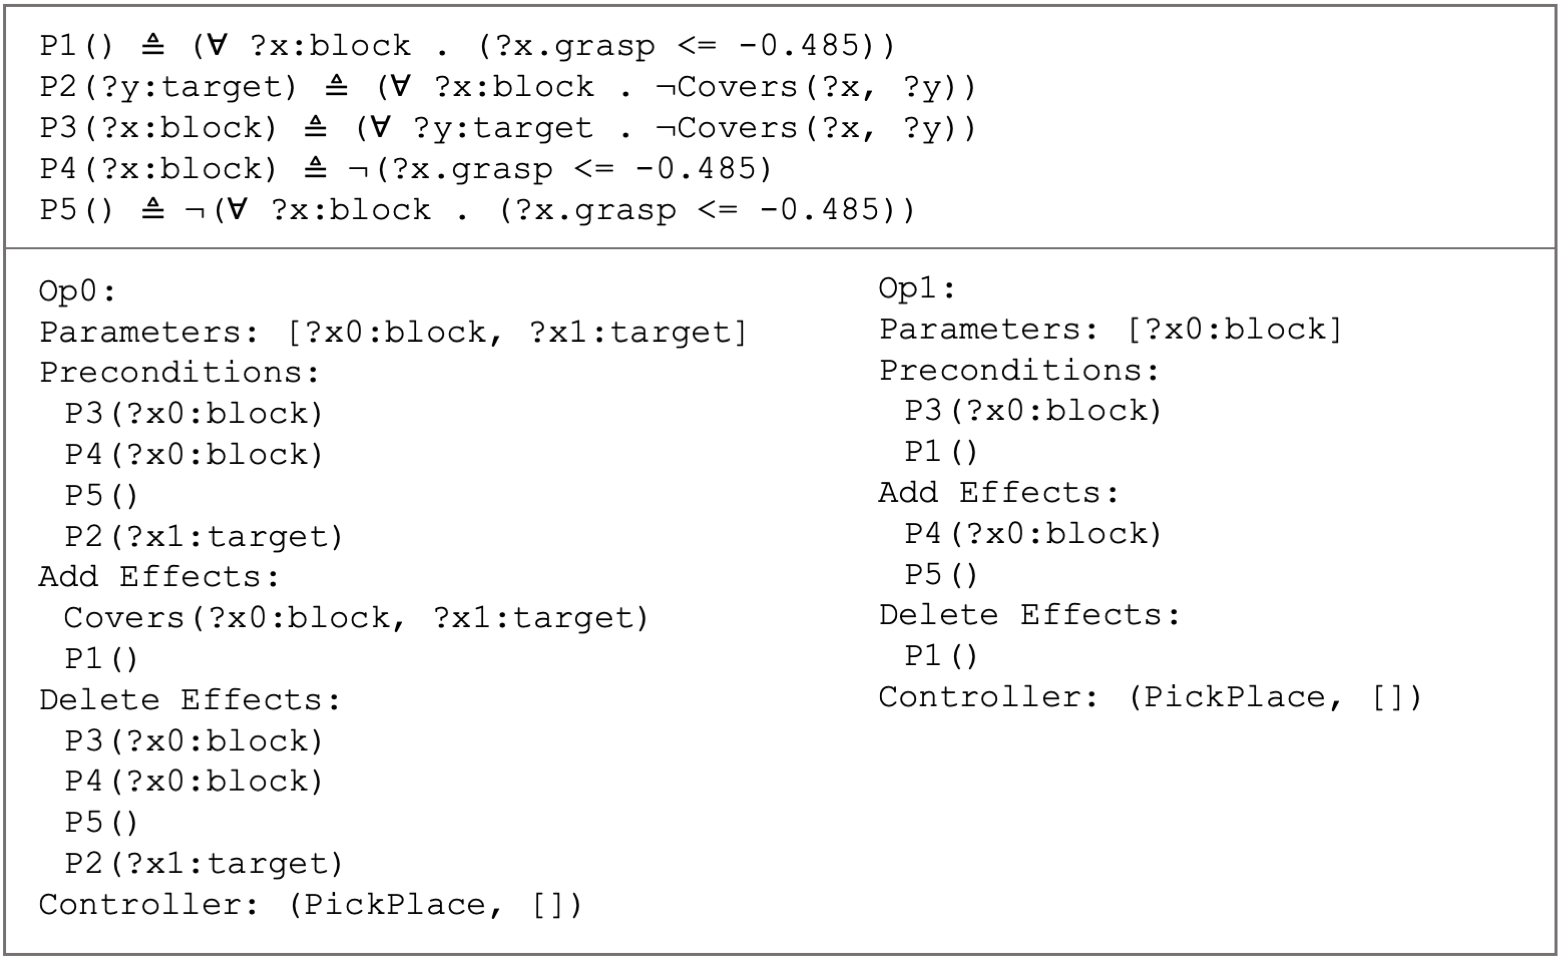
\includegraphics[width=0.95\textwidth]{figures/pickplace1d_learned.png}
    \caption{PickPlace1D learned abstractions (top: predicates, bottom: operators).}
  \label{fig:pickplace1dlearned}
\end{figure*}


\begin{figure*}[t]
  \centering
    \noindent
    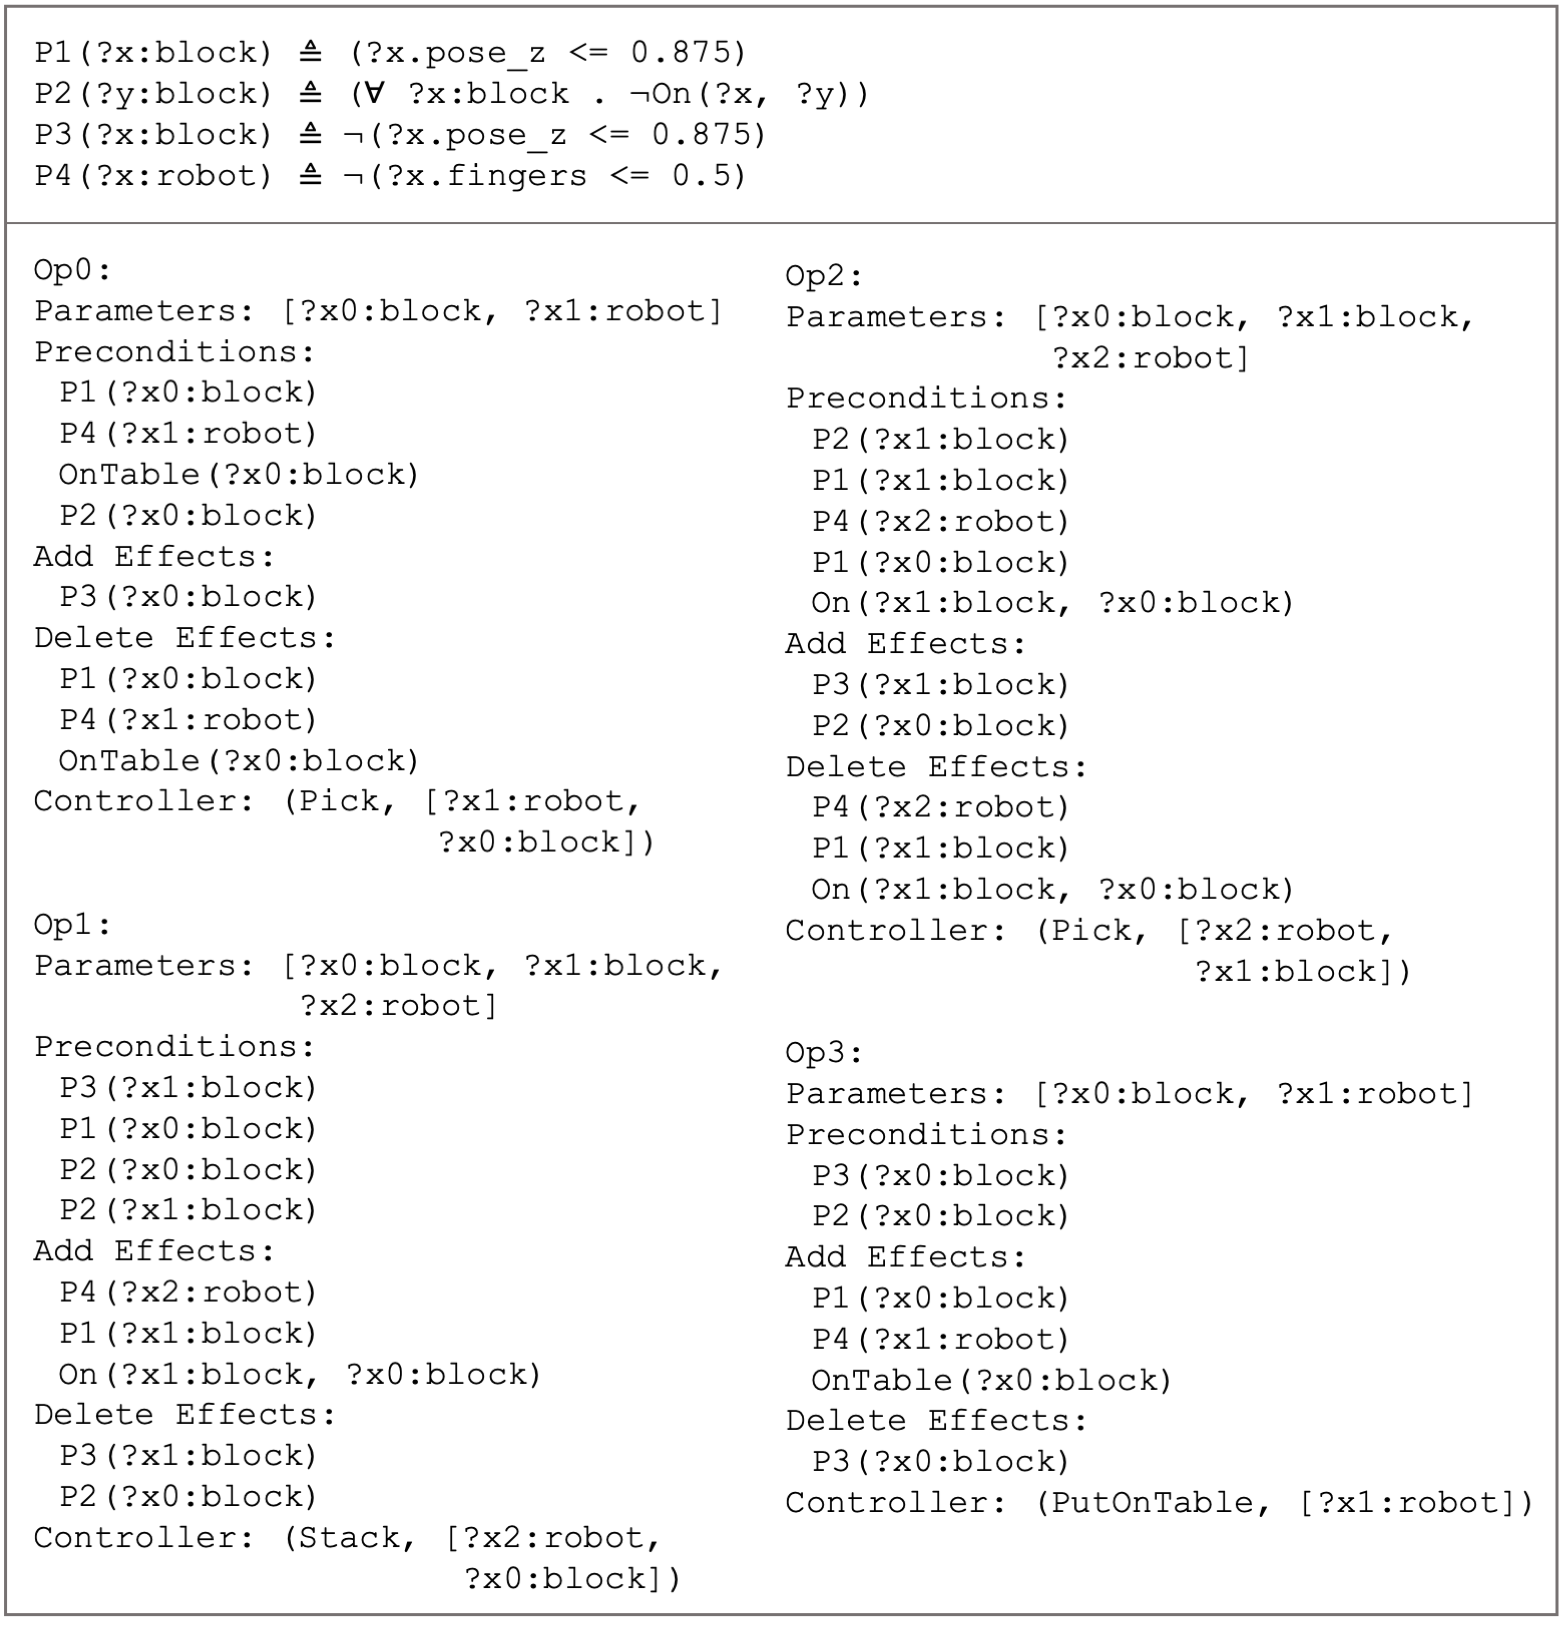
\includegraphics[width=0.95\textwidth]{figures/blocks_learned.png}
    \caption{Blocks learned abstractions (top: predicates, bottom: operators).}
  \label{fig:blockslearned}
\end{figure*}


\begin{figure*}[t]
  \centering
    \noindent
    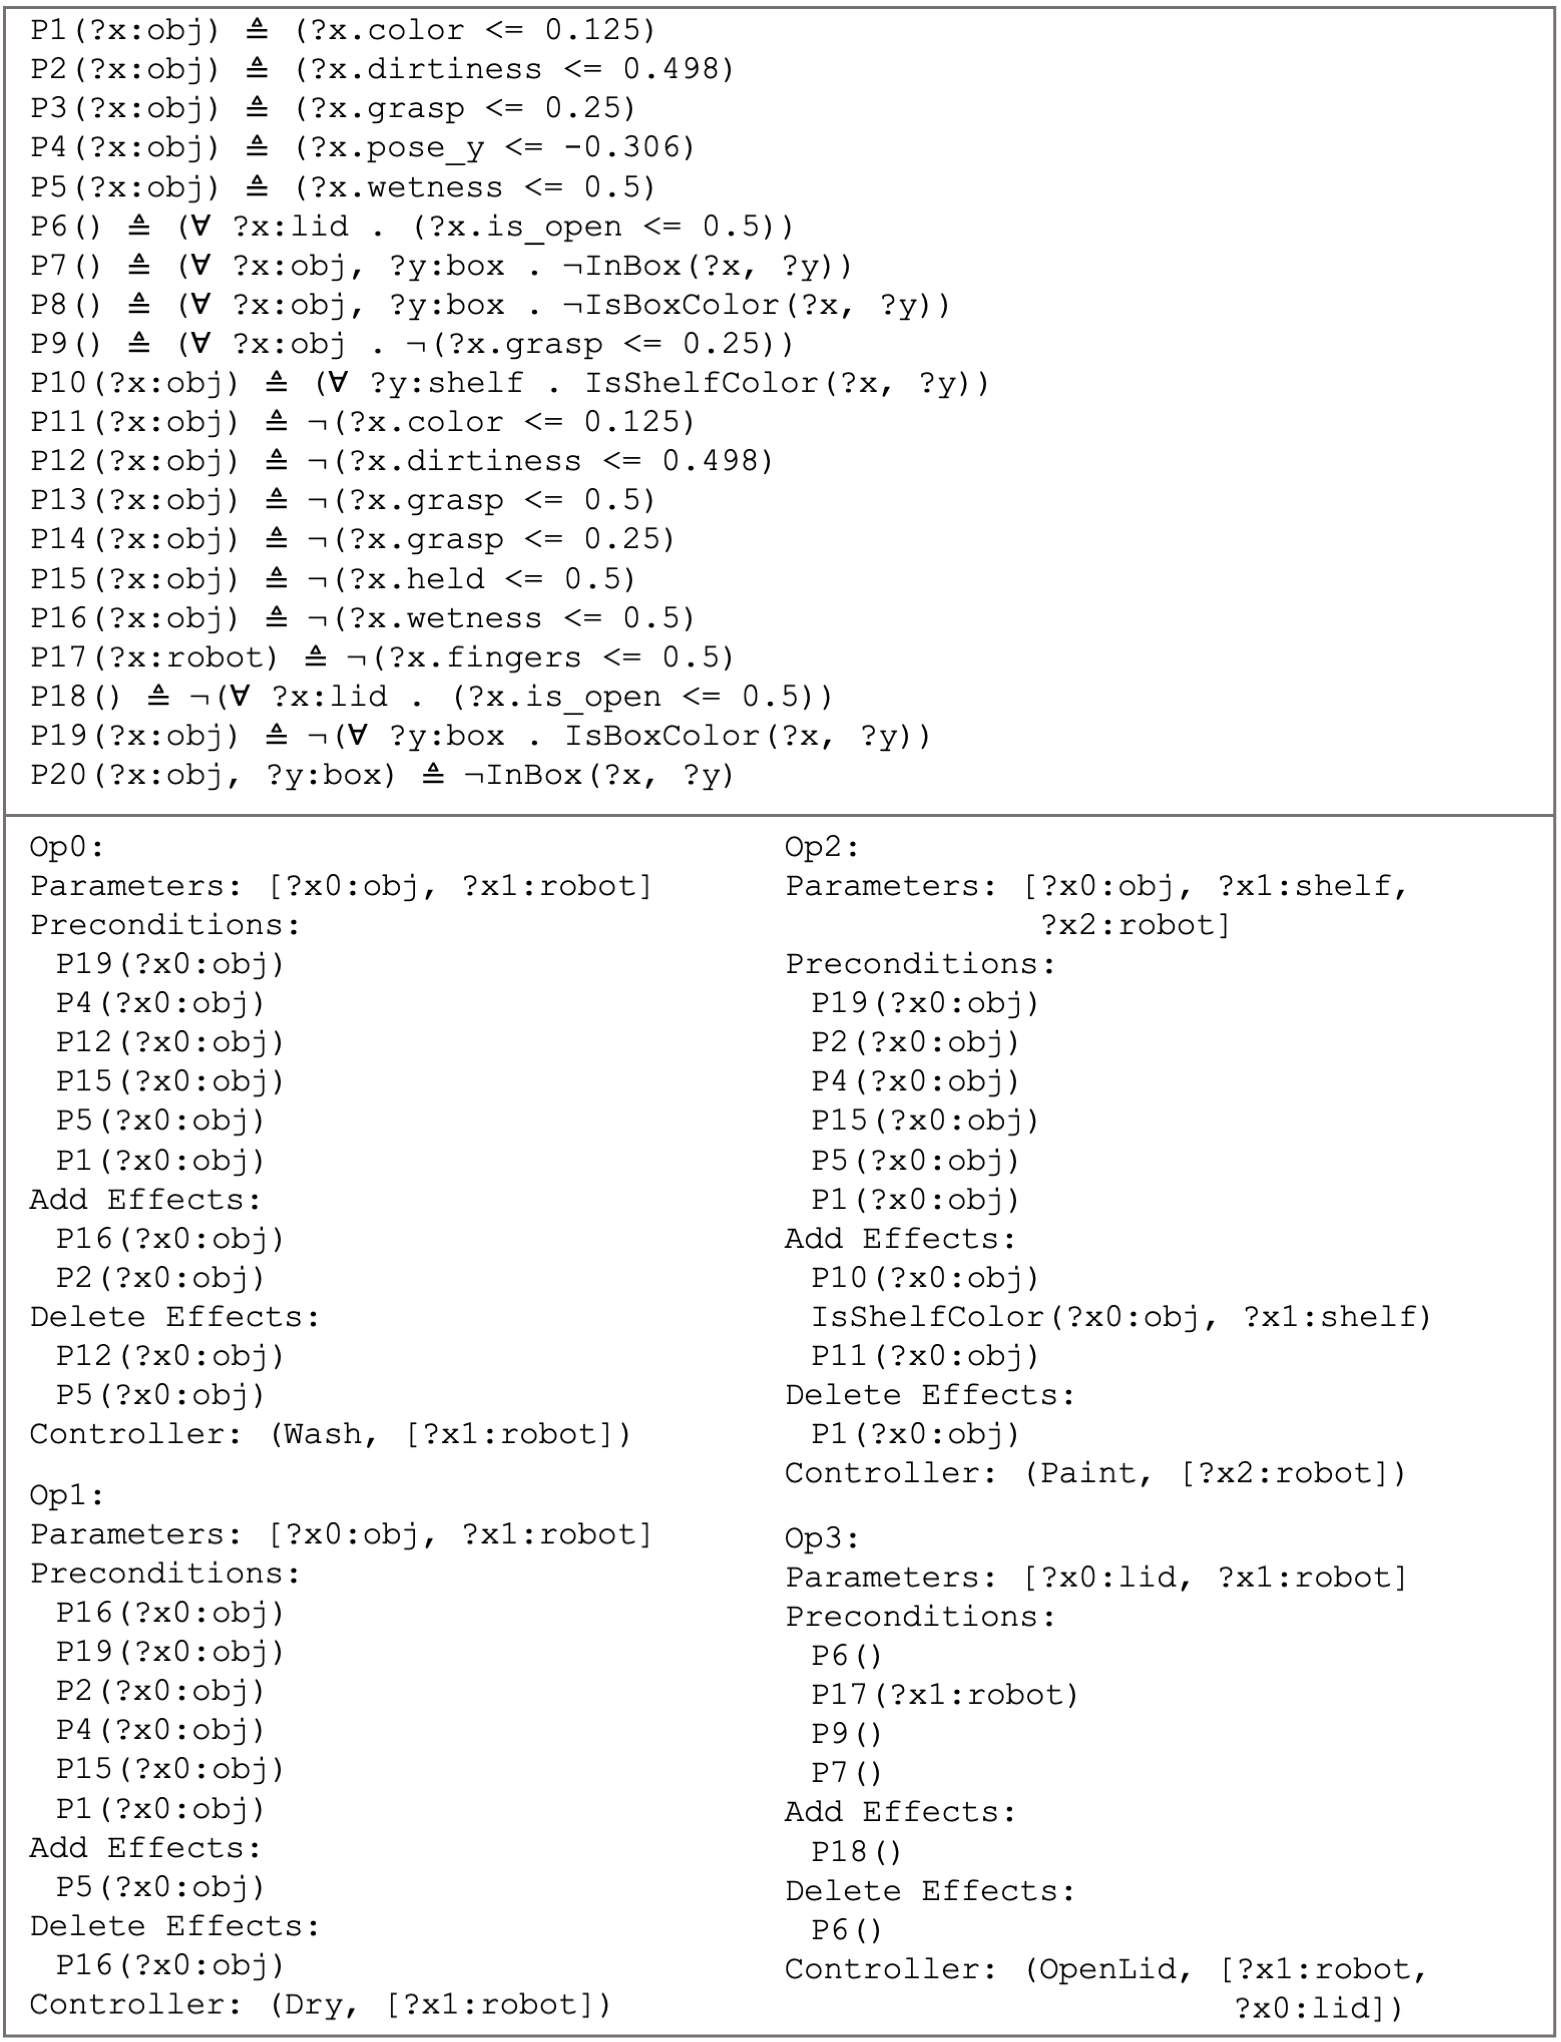
\includegraphics[width=0.95\textwidth]{figures/painting_learned1.png}
    \caption{Painting learned abstractions (top: predicates, bottom: operators part 1 of 2).}
  \label{fig:paintinglearned1}
\end{figure*}

\begin{figure*}[t]
  \centering
    \noindent
    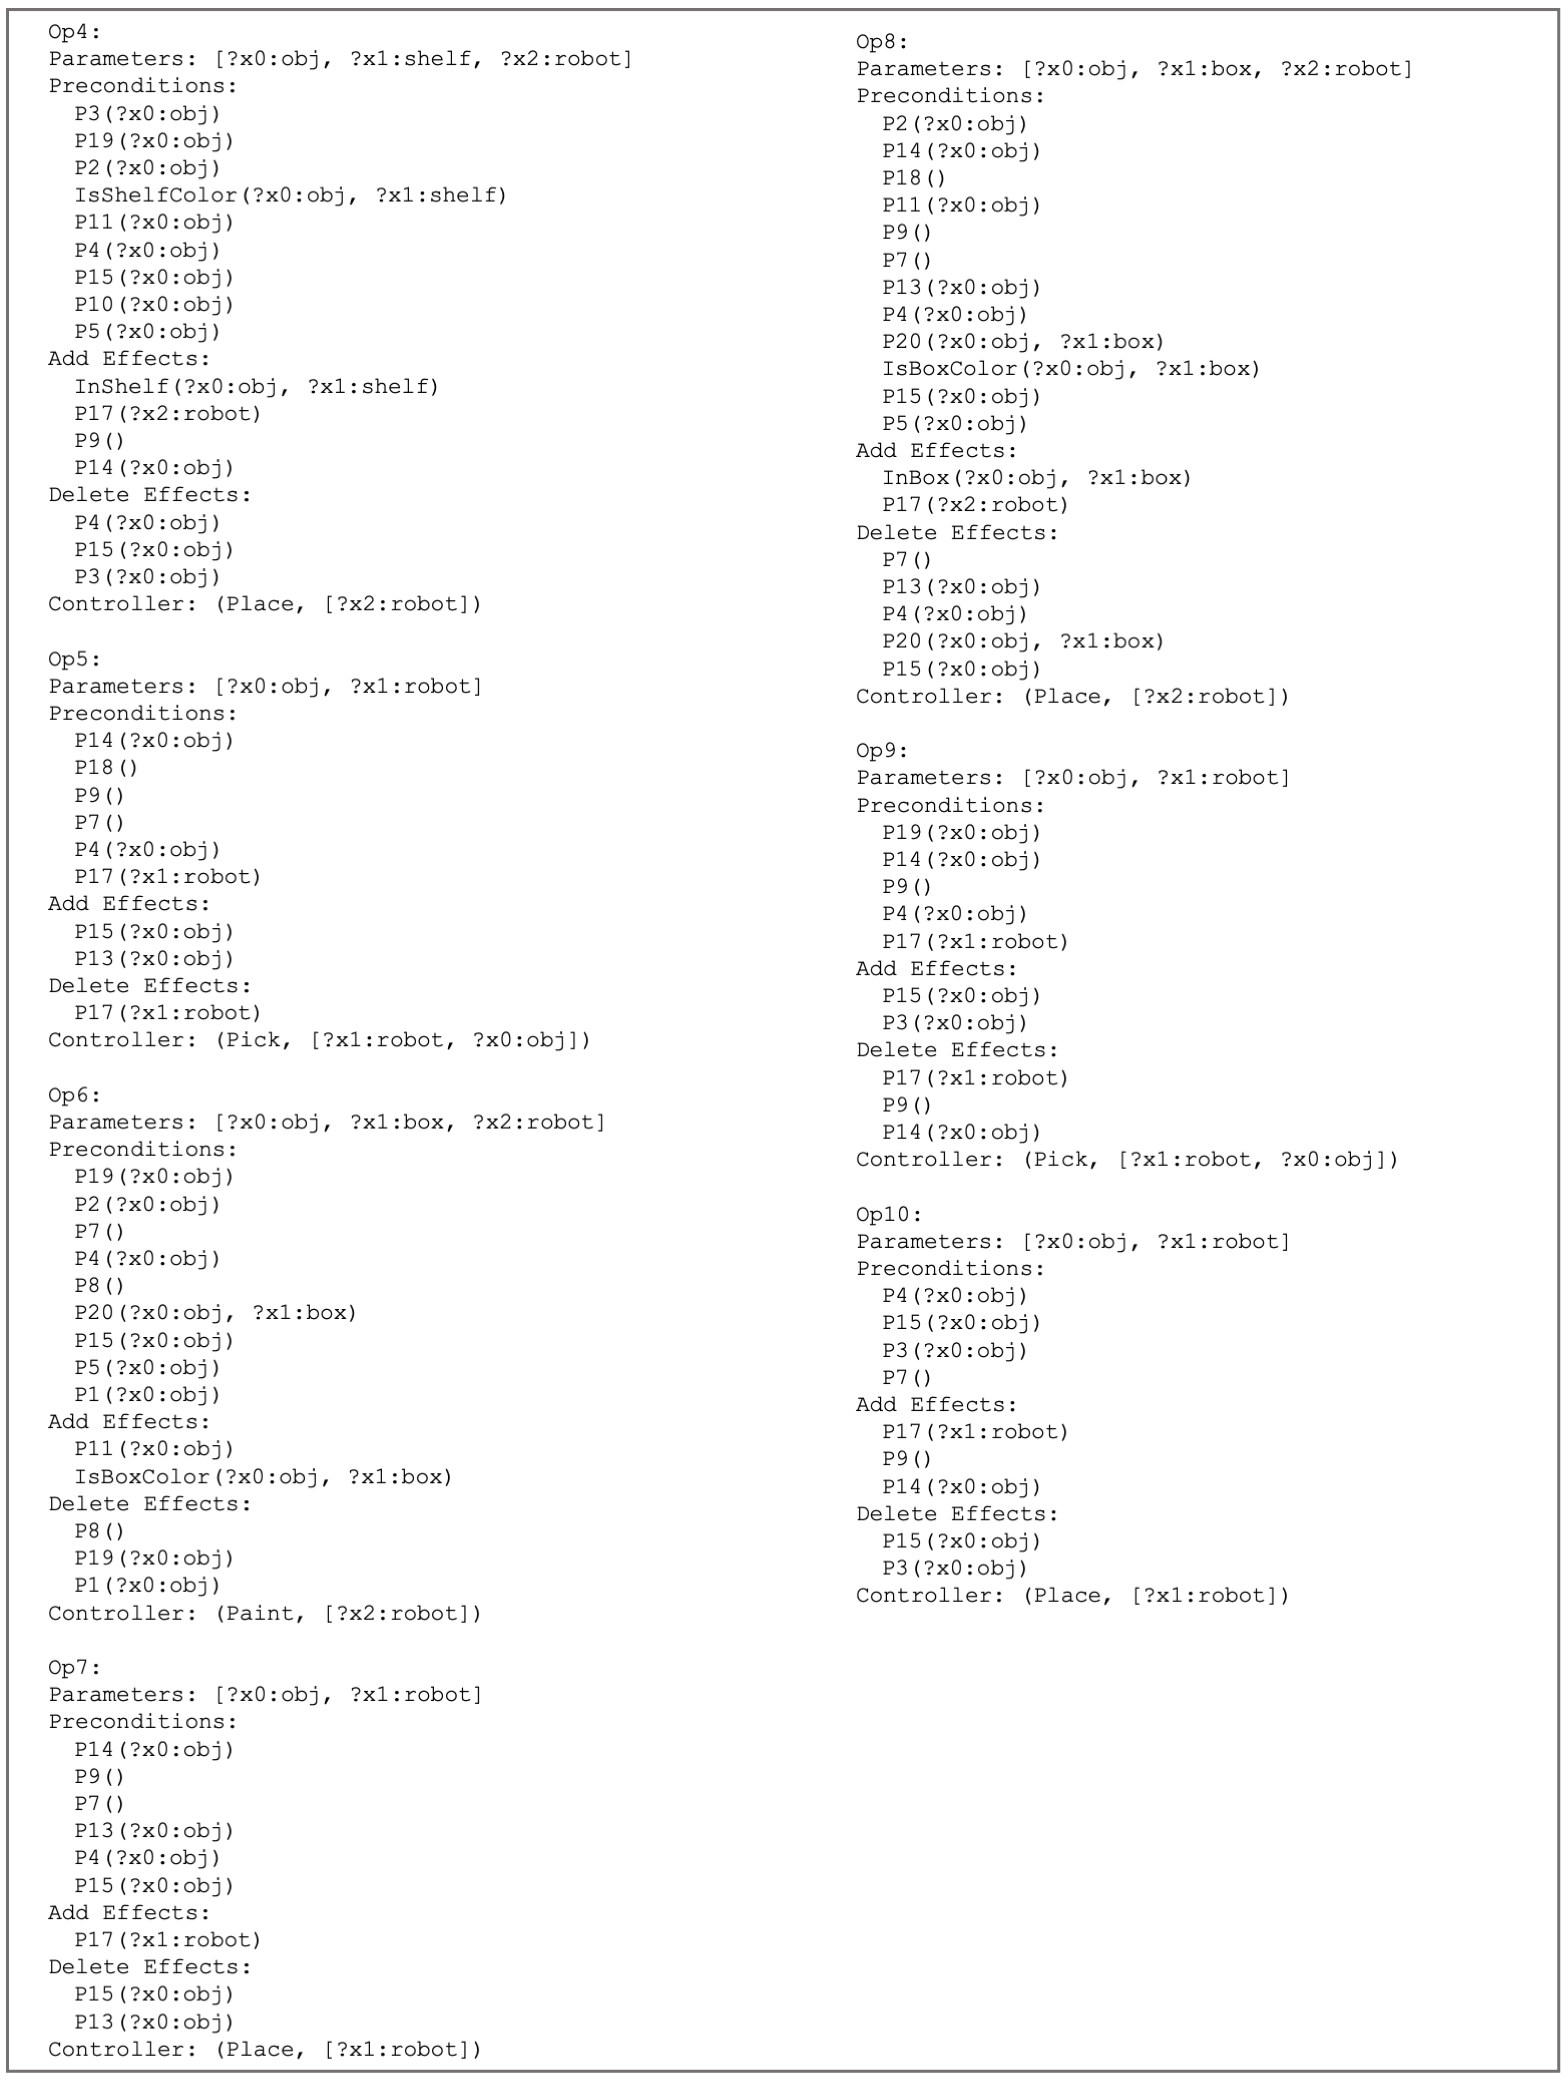
\includegraphics[width=0.93\textwidth]{figures/painting_learned2.png}
    \caption{Painting learned abstractions (operators part 2 of 2).}
  \label{fig:paintinglearned2}
\end{figure*}

\begin{figure*}[t]
  \centering
    \noindent
    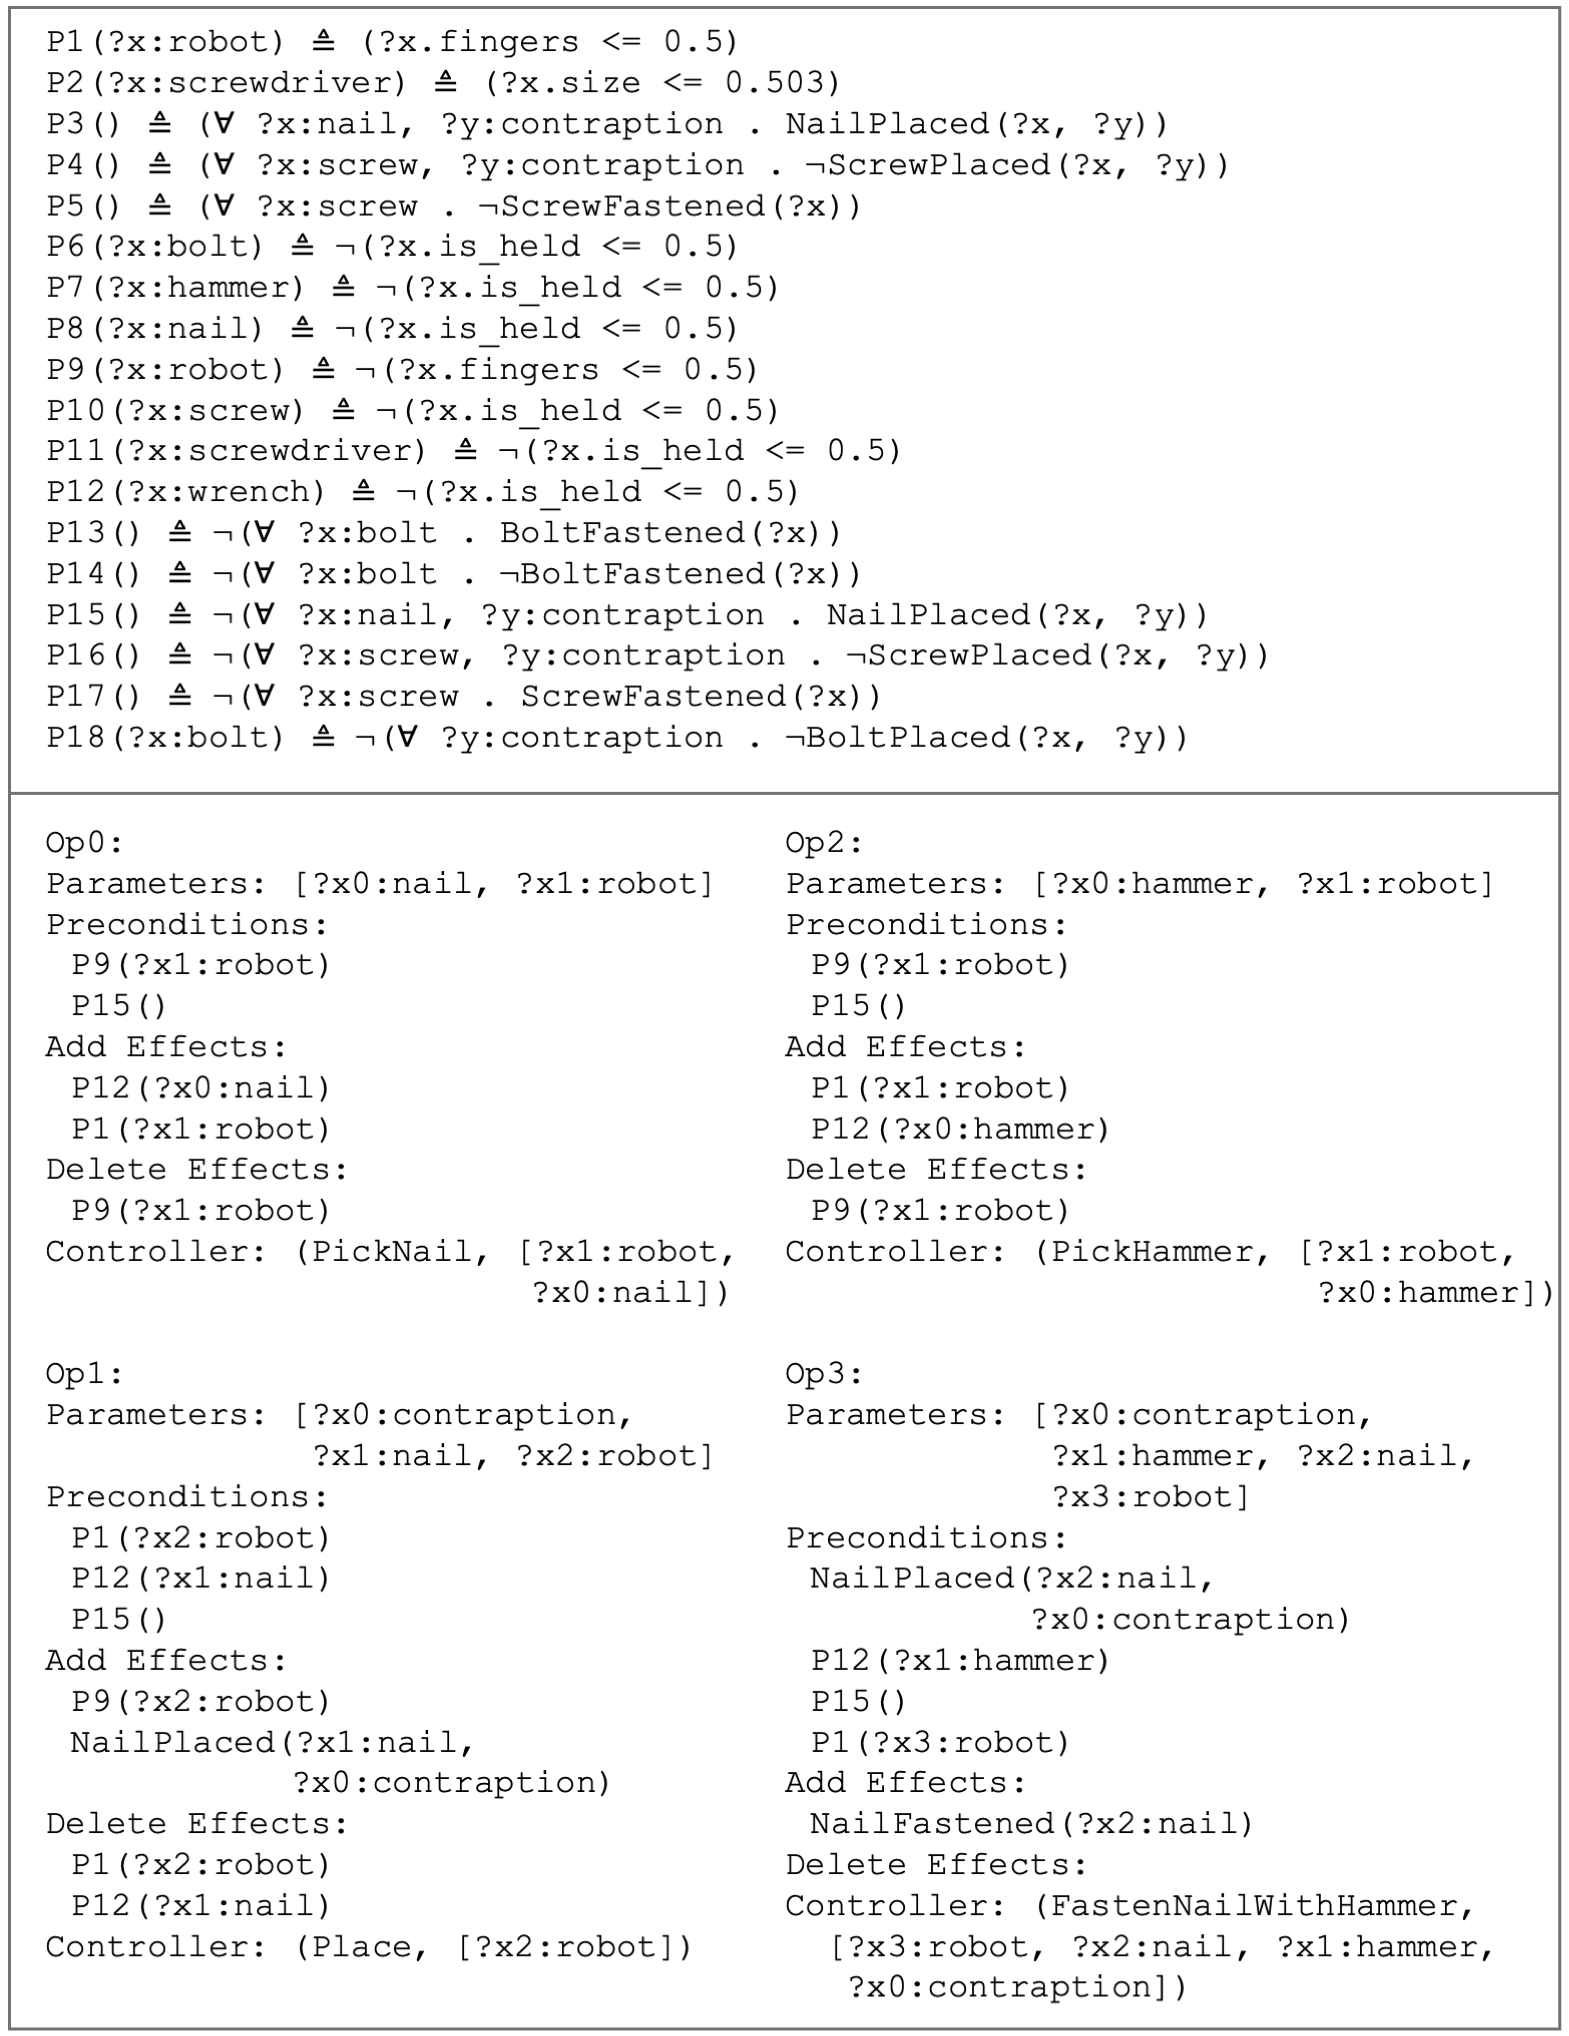
\includegraphics[width=0.95\textwidth]{figures/tools_learned1.png}
    \caption{Tools learned abstractions (top: predicates, bottom: operators part 1 of 2).}
  \label{fig:toolslearned1}
\end{figure*}

\begin{figure*}[t]
  \centering
    \noindent
    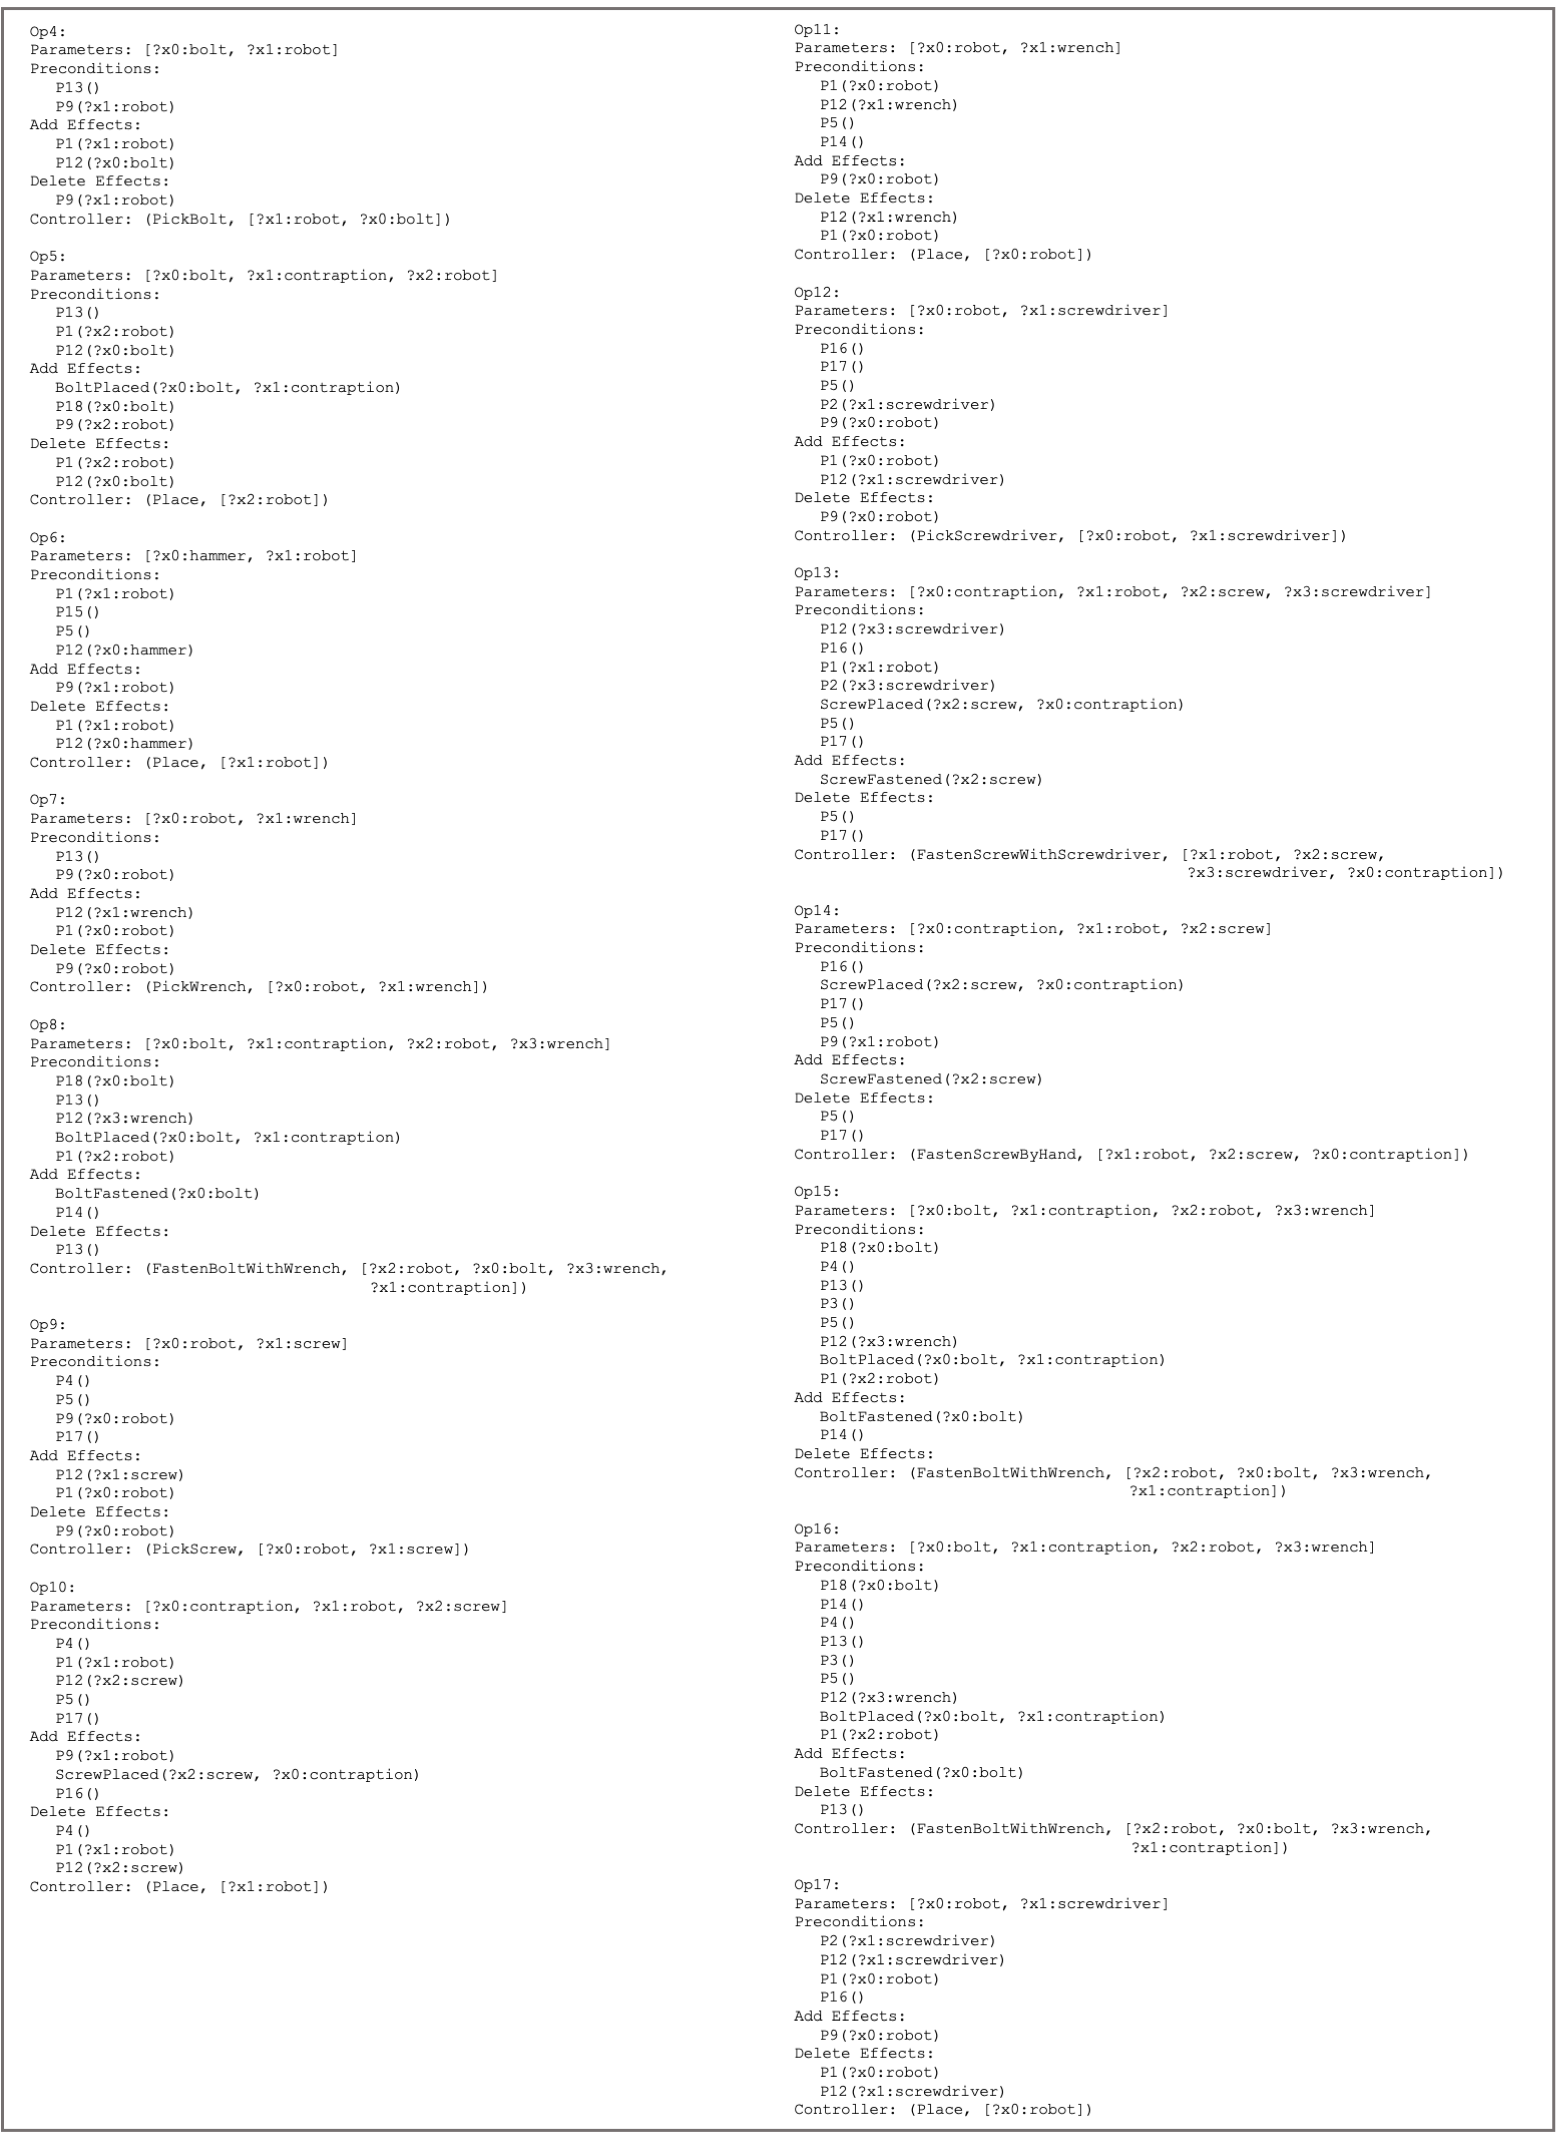
\includegraphics[width=0.9\textwidth]{figures/tools_learned2.png}
    \caption{Tools learned abstractions (operators part 2 of 2).}
  \label{fig:toolslearned2}
\end{figure*}
